% =============================================================================
% relatorio_alu_bw.tex -- Relatorio Tecnico: ALUChip v1.0 (versao preto/branco)
% Unidade 7 | Capitulo 5 | Desafio de Design de CIs -- PADIS
% Autor  : Romulo da Silva Lira
% Prof.  : Andre Feitosa (CI Amazônia)
% =============================================================================
\documentclass[12pt,a4paper]{article}

\usepackage[utf8]{inputenc}
\usepackage[T1]{fontenc}
\usepackage[brazil]{babel}
\usepackage{lmodern}
\usepackage{microtype}
\usepackage{geometry}
% Margens ABNT (NBR 14724): esq=3cm, dir=2cm, sup=3cm, inf=2cm
\geometry{top=3cm,bottom=2cm,left=3cm,right=2cm,headheight=14pt}
\usepackage{setspace}
\onehalfspacing
\usepackage{graphicx}
\usepackage[table]{xcolor}
\usepackage{tikz}
\usetikzlibrary{shapes.geometric,arrows.meta,positioning,fit,calc,decorations.pathreplacing}
\usepackage{pgfplots}
\pgfplotsset{compat=1.18}
\usepackage{booktabs,multirow,array,longtable,colortbl}
\usepackage{listings,caption,subcaption}
\usepackage{amsmath,amssymb,mathtools,bm}
\usepackage{fancyhdr,titlesec,setspace,parskip,enumitem}
\usepackage[most]{tcolorbox}
\tcbuselibrary{listings,breakable,skins}
\usepackage[hidelinks,pdftitle={ALUChip v1.0},pdfauthor={Romulo da Silva Lira}]{hyperref}
\usepackage{siunitx}
\sisetup{output-decimal-marker={,},group-separator={.}}

% ── Paleta Preto/Branco ───────────────────────────────────────────────────────
\definecolor{bwblack}{RGB}{20,20,20}
\definecolor{bwdark}{RGB}{60,60,60}
\definecolor{bwgray}{RGB}{110,110,110}
\definecolor{bwlight}{RGB}{242,242,242}
\definecolor{bwcode}{RGB}{248,248,248}

% ── Listagem SystemVerilog (P/B) ──────────────────────────────────────────────
\lstdefinelanguage{SystemVerilog}{
  morekeywords={module,endmodule,input,output,logic,wire,reg,always_comb,
    assign,begin,end,case,endcase,default,if,else,parameter,localparam,
    task,endtask,automatic,initial,$dumpfile,$dumpvars,$display,$finish,int,
    timescale,string},
  sensitive=true,
  morecomment=[l]{//},
  morestring=[b]",
}
\lstdefinestyle{svstyle}{
  language=SystemVerilog,
  basicstyle=\ttfamily\small,
  keywordstyle=\color{bwblack}\bfseries,
  commentstyle=\color{bwgray}\itshape,
  numbers=left, numberstyle=\tiny\color{bwgray}, stepnumber=1, numbersep=8pt,
  frame=single, framerule=0.6pt, rulecolor=\color{bwdark},
  backgroundcolor=\color{bwcode},
  breaklines=true, showstringspaces=false, tabsize=4, captionpos=b,
  xleftmargin=15pt, xrightmargin=5pt,
}

% ── Caixas (P/B) ─────────────────────────────────────────────────────────────
\newtcolorbox{unidadebox}[1][]{enhanced,colback=bwlight,colframe=bwdark,
  coltitle=white,fonttitle=\bfseries\normalsize,title={#1},boxrule=1.2pt,
  arc=4pt,left=8pt,right=8pt,top=6pt,bottom=6pt,breakable}
\newtcolorbox{resultbox}[1][]{enhanced,colback=bwlight,
  colframe=bwblack,coltitle=white,fonttitle=\bfseries\small,
  title={#1},boxrule=1pt,arc=3pt,left=6pt,right=6pt,top=5pt,bottom=5pt,breakable}
\newtcolorbox{specbox}[1][]{enhanced,colback=bwlight,colframe=bwgray,
  coltitle=bwblack,fonttitle=\bfseries\small,title={#1},
  boxrule=0.8pt,arc=3pt,left=6pt,right=6pt,top=5pt,bottom=5pt,breakable}

% ── Cabecalho P/B ─────────────────────────────────────────────────────────────
\pagestyle{fancy}\fancyhf{}
\fancyhead[L]{\small\textbf{ALUChip v1.0} --- ULA 8 bits}
\fancyhead[R]{\small PADIS $|$ Unidade~7 $|$ Cap.~5}
\fancyfoot[L]{\small R\^{o}mulo da Silva Lira --- CI Amaz\^{o}nia}
\fancyfoot[C]{\small\thepage}
\fancyfoot[R]{\small Prof.\ Andr\'{e} Feitosa}
\renewcommand{\headrulewidth}{0.6pt}
\renewcommand{\footrulewidth}{0.4pt}

% ── Titulos P/B ──────────────────────────────────────────────────────────────
\titleformat{\section}{\large\bfseries\color{bwblack}}{\thesection.}{0.6em}{}
  [\vspace{-4pt}\textcolor{bwdark}{\hrule height 0.6pt}\vspace{2pt}]
\titleformat{\subsection}{\normalsize\bfseries\color{bwdark}}{\thesubsection.}{0.5em}{}
\titleformat{\subsubsection}{\normalsize\bfseries\color{bwgray}}{\thesubsubsection.}{0.4em}{}

% =============================================================================
\begin{document}
\thispagestyle{empty}

% ── Capa (NBR 14724) ────────────────────────────────────────────────────
\begin{center}
  \vspace*{0.5cm}
  
\includegraphics[height=1.8cm]{softex_logo.jpg}\hspace{1.2cm}%
  \raisebox{0.5cm}{\normalsize\bfseries CI Amazônia --- Capacitação em Microeletrônica}\\[18pt]
  {\normalsize Projeto de An\'{a}lise e Design de Sistemas Integrados -- PADIS}\\[40pt]

  {\LARGE\bfseries ALUChip v1.0}\\[10pt]
  {\large\bfseries Unidade L\'{o}gico-Aritm\'{e}tica de 8~Bits}\\[6pt]
  {\normalsize\color{bwgray}
    8~Opera\c{c}\~{o}es $|$ 4~\textit{Flags} $|$ CMOS 0,35\,\textmu m $|$ VDD\,=\,3,3\,V}\\[40pt]

  {\normalsize\bfseries R\^{o}mulo da Silva Lira}\\[60pt]

  \vfill
  {\normalsize\textbf{Orientador:} Prof.\ Andr\'{e} Feitosa}\\[6pt]
  {\normalsize Unidade~7 --- Cap\'{\i}tulo~5 | Desafio de Design de Circuitos Integrados}\\[6pt]
  {\normalsize Manaus -- AM}\\[4pt]
  {\normalsize \the\year}
\end{center}

\newpage
\thispagestyle{empty}
\begin{center}
  \vspace*{0.5cm}
  {\normalsize\bfseries CI Amazônia --- Capacitação em Microeletrônica}\\[3pt]
  {\normalsize\bfseries Instituto de Computa\c{c}\~{a}o -- ICOMP}\\[30pt]

  {\normalsize\bfseries R\^{o}mulo da Silva Lira}\\[40pt]

  {\LARGE\bfseries ALUChip v1.0}\\[10pt]
  {\large\bfseries Unidade L\'{o}gico-Aritm\'{e}tica de 8~Bits}\\[40pt]

  \begin{minipage}{0.55\textwidth}
  \begin{flushright}
    {\small Relatório técnico apresentado como entrega do Desafio de Design de Circuitos Integrados na disciplina PADIS --- Unidade~7, Capítulo~5.}\\[10pt]
    {\small \textbf{Orientador:} Prof.\ Andr\'{e} Feitosa}
  \end{flushright}
  \end{minipage}\\[60pt]

  \vfill
  {\normalsize Manaus -- AM}\\[4pt]
  {\normalsize \the\year}
\end{center}

\newpage\thispagestyle{empty}\vspace*{3cm}
\begin{center}
  \begin{tabular}{rl}
    \textbf{Autor:}      & R\^{o}mulo da Silva Lira \\
    \textbf{Professor:}  & Andr\'{e} Feitosa \\
    \textbf{Programa:}& CI Amaz\^{o}nia / Softex \\
    \textbf{Disciplina:} & PADIS --- Unidade~7, Cap\'{\i}tulo~5 \\
    \textbf{Entrega:}    & Desafio de Design de Circuitos Integrados \\
    \textbf{Data:}       & \today \\
  \end{tabular}
\end{center}
\vspace{1cm}
\begin{center}

  % Diagrama de blocos top-level (P/B)
  \begin{tikzpicture}[
    box/.style={draw=bwdark,fill=bwlight,rounded corners=4pt,
                minimum width=2.4cm,minimum height=1.1cm,align=center,
                font=\small\bfseries},
    mux/.style={draw=bwblack,fill=bwlight,rounded corners=2pt,
                minimum width=1.4cm,minimum height=2.4cm,align=center,
                font=\small\bfseries},
    arr/.style={-{Stealth[scale=1.1]},thick,color=bwdark}
  ]
    \node[box] (add) at (0,1.2) {Adder\\ADD/SUB};
    \node[box] (log) at (0,0) {Logic\\AND$\cdot$OR$\cdot$XOR$\cdot$NOT};
    \node[box] (shf) at (0,-1.2) {Shifter\\SHL$\cdot$SHR};
    \node[mux] (mux) at (3.2,0) {MUX\\8:1};
    \node[box] (flg) at (6.0,0) {Flags\\Z$\cdot$C$\cdot$V$\cdot$N};
    \draw[arr] (add.east) -- (mux.west|-add.east);
    \draw[arr] (log.east) -- (mux.west);
    \draw[arr] (shf.east) -- (mux.west|-shf.east);
    \draw[arr] (mux.east) -- node[above,font=\tiny\ttfamily]{RESULT[7:0]} (flg.west);
    \draw[arr] (flg.east) -- ++(1.2,0) node[right,font=\tiny\ttfamily]{Z C V N};
    \node[left=1.5cm of add,font=\tiny\ttfamily] (ia) {A[7:0]};
    \draw[arr] (ia.east) -- (add.west);
    \draw[arr] (ia.east|-log.west) -- (log.west);
    \draw[arr] (ia.east|-shf.west) -- (shf.west);
    \node[below=0.5cm of mux,font=\tiny\ttfamily] {OP[2:0]};
    \draw[arr] (3.2,-0.9) -- (mux.south);
  \end{tikzpicture}

  \vfill
  {\small Simula\c{c}\~{a}o funcional: \textbf{27/27 testes aprovados} (Icarus Verilog v12)}
\end{center}

\newpage

% ── Resumo ───────────────────────────────────────────────────────────────────
\begin{center}{\large\bfseries Resumo}\end{center}
\begin{unidadebox}[Resumo]
Este trabalho descreve o projeto completo do \textbf{ALUChip v1.0}, uma Unidade L\'{o}gico-Aritm\'{e}tica (ULA) de 8~bits com 8~opera\c{c}\~{o}es e 4~flags de estado, implementada em processo CMOS 0,35\,\textmu m com tens\~{a}o de alimenta\c{c}\~{a}o de 3,3\,V. O circuito executa opera\c{c}\~{o}es aritm\'{e}ticas (\texttt{ADD}, \texttt{SUB}), l\'{o}gicas (\texttt{AND}, \texttt{OR}, \texttt{XOR}, \texttt{NOT}) e de deslocamento (\texttt{SHL}, \texttt{SHR}) selecionadas por um c\'{o}digo de 3~bits, produzindo um resultado de 8~bits e quatro sinalizadores: \textit{Zero}~(Z), \textit{Carry}~(C), \textit{Overflow}~(V) e \textit{Negativo}~(N). A l\'{o}gica \'{e} inteiramente combinacional. A verifica\c{c}\~{a}o funcional com Icarus Verilog v12 obteve \textbf{aprova\c{c}\~{a}o em 27/27 vetores de teste}. O fluxo completo inclui descri\c{c}\~{a}o RTL (SystemVerilog), simula\c{c}\~{a}o funcional com \textit{golden model}, \textit{layout} f\'{\i}sico CMOS, extra\c{c}\~{a}o de par\'{a}sitas RC, simula\c{c}\~{a}o p\'{o}s-\textit{layout} e verifica\c{c}\~{a}o LVS/DRC.\\[4pt]
\textbf{Palavras-chave:} ULA; ALU; 8~bits; l\'{o}gica combinacional; CMOS 0,35\,\textmu m; flags; SystemVerilog; LVS; extra\c{c}\~{a}o de par\'{a}sitas.
\end{unidadebox}

\vspace{6pt}
\begin{center}{\large\bfseries Abstract}\end{center}
\begin{unidadebox}[Abstract]
This paper presents the complete design of \textbf{ALUChip v1.0}, an 8-bit Arithmetic Logic Unit (ALU) featuring 8 operations and 4 status flags, targeting a CMOS 0.35\,\textmu m process at 3.3\,V supply. The circuit performs arithmetic (\texttt{ADD}, \texttt{SUB}), logic (\texttt{AND}, \texttt{OR}, \texttt{XOR}, \texttt{NOT}), and shift (\texttt{SHL}, \texttt{SHR}) operations selected by a 3-bit opcode, delivering an 8-bit result and four flags: \textit{Zero}~(Z), \textit{Carry}~(C), \textit{Overflow}~(V), and \textit{Negative}~(N). The all-combinational datapath was verified at 27/27 test vectors and subjected to the full ASIC flow: RTL, functional simulation, physical layout, RC parasitics extraction, post-layout simulation, and LVS/DRC sign-off.\\[4pt]
\textbf{Keywords:} ALU; 8-bit; combinational logic; CMOS 0.35\,\textmu m; status flags; SystemVerilog; LVS; parasitic extraction.
\end{unidadebox}

\newpage
\tableofcontents
\listoffigures
\listoftables
\newpage

% =============================================================================
\section{Introdu\c{c}\~{a}o}
% =============================================================================

A Unidade L\'{o}gico-Aritm\'{e}tica (ULA, ou \textit{Arithmetic Logic Unit} --- ALU) \'{e} o bloco funcional mais fundamental de qualquer processador digital. Proposta na forma moderna por John von Neumann em seu relat\'{o}rio de 1945~\cite{vonneumann1945} e concretizada em sil\'{\i}cio no Intel 4004 (1971)~\cite{intel4004}, a ALU executa opera\c{c}\~{o}es matem\'{a}ticas e l\'{o}gicas sobre dados bin\'{a}rios, produzindo sinalizadores de estado (\textit{flags}) que controlam o fluxo do programa por meio de instru\c{c}\~{o}es de desvio condicional.

\begin{unidadebox}[Import\^{a}ncia Hist\'{o}rica e Industrial da ALU]
\begin{itemize}[leftmargin=1.5em]
  \item \textbf{Intel 4004 (1971):} primeira ALU de 4~bits em um \'{u}nico CI, 2.300 transistores, processo 10\,\textmu m.
  \item \textbf{Intel 8080 (1974):} ALU de 8~bits, base do CP/M e do MS-DOS; mesmo tamanho de dados do ALUChip v1.0.
  \item \textbf{ARMv7/v8:} ALU de 32/64~bits com suporte a SIMD; toda instru\c{c}\~{a}o aritm\'{e}tica passa por um bloco equivalente ao projetado aqui.
  \item \textbf{RISC-V (2010--):} ISA aberta com ALU de 32/64~bits; o conjunto m\'{\i}nimo RV32I usa exatamente ADD, SUB, AND, OR, XOR e deslocamentos --- as mesmas 8~opera\c{c}\~{o}es do ALUChip v1.0.
\end{itemize}
\end{unidadebox}

O \textbf{ALUChip v1.0} implementa uma ULA de 8~bits com as 8~opera\c{c}\~{o}es fundamentais do repert\'{o}rio RISC, em processo CMOS 0,35\,\textmu m com 3,3\,V. O design \'{e} inteiramente combinacional, garantindo zero lat\^{e}ncia de \textit{pipeline} para integra\c{c}\~{a}o em caminhos de dados cr\'{\i}ticos de microcontroladores e sistemas embarcados.

Este relat\'{o}rio cobre o fluxo completo de projeto: especifica\c{c}\~{a}o, RTL SystemVerilog, simula\c{c}\~{a}o funcional (\textit{golden model}), \textit{layout} f\'{\i}sico CMOS, extra\c{c}\~{a}o de par\'{a}sitas RC, simula\c{c}\~{a}o p\'{o}s-\textit{layout} e verifica\c{c}\~{a}o LVS/DRC, contemplando os 7~pontos obrigat\'{o}rios do Desafio de Design de CIs da Unidade~7.

% =============================================================================
\section{Metodologia}
% =============================================================================

\subsection{Especifica\c{c}\~{a}o das Opera\c{c}\~{o}es}

A Tabela~\ref{tab:ops} define formalmente as 8~opera\c{c}\~{o}es implementadas, o c\'{o}digo de 3~bits e o comportamento das \textit{flags}.

\begin{table}[h!]
\centering
\caption{Tabela de opera\c{c}\~{o}es do ALUChip v1.0}
\label{tab:ops}
\rowcolors{2}{bwlight}{white}
\begin{tabular}{c c l l l}
\toprule
\textbf{OP[2:0]} & \textbf{Mnem\^{o}nico} & \textbf{Opera\c{c}\~{a}o} & \textbf{Flags atualizadas} & \textbf{Aplica\c{c}\~{a}o t\'{\i}pica} \\
\midrule
\texttt{000} & ADD  & $\text{R} = A + B$         & Z, C, V, N & Adi\c{c}\~{a}o inteira \\
\texttt{001} & SUB  & $\text{R} = A - B$         & Z, C, V, N & Subtra\c{c}\~{a}o / compara\c{c}\~{a}o \\
\texttt{010} & AND  & $\text{R} = A \land B$     & Z, N       & M\'{a}scara de bits \\
\texttt{011} & OR   & $\text{R} = A \lor B$      & Z, N       & Set de bits \\
\texttt{100} & XOR  & $\text{R} = A \oplus B$    & Z, N       & Toggle / compara\c{c}\~{a}o \\
\texttt{101} & NOT  & $\text{R} = \overline{A}$  & Z, N       & Invers\~{a}o (B ignorado) \\
\texttt{110} & SHL  & $\text{R} = A \ll 1,\ C = A_7$ & Z, C, N  & Multiplica por 2 \\
\texttt{111} & SHR  & $\text{R} = A \gg 1,\ C = A_0$ & Z, C, N  & Divide por 2 \\
\bottomrule
\end{tabular}
\end{table}

\subsection{Sem\^{a}ntica das Flags}

As 4~\textit{flags} de estado s\~{a}o definidas formalmente:

\begin{align}
  Z &= (R[7:0] = \texttt{0x00})
    \qquad\text{(NOR de todos os 8~bits do resultado)} \label{eq:z}\\
  C &= \text{carry-out}_{[8]} \text{ (ADD/SUB)}
     \;|\; A_7 \text{ (SHL)}
     \;|\; A_0 \text{ (SHR)} \label{eq:c}\\
  V &= (\overline{A_7} \cdot \overline{B_7} \cdot R_7) \lor (A_7 \cdot B_7 \cdot \overline{R_7})
    \quad\text{(ADD); sinal trocado (SUB)} \label{eq:v}\\
  N &= R[7]
    \qquad\text{(MSB do resultado, indica n\'{u}mero negativo em C2)} \label{eq:n}
\end{align}

\subsection{Fluxo de Design}

O fluxo de projeto seguiu as etapas abaixo, contemplando os 7~pontos obrigat\'{o}rios do desafio:

\begin{enumerate}[leftmargin=2em,label=\textbf{E\arabic*.}]
  \item Especifica\c{c}\~{a}o formal das opera\c{c}\~{o}es e sem\^{a}ntica de \textit{flags}.
  \item Implementa\c{c}\~{a}o RTL em SystemVerilog IEEE 1800-2012 (\textbf{Ponto~1 e~2}).
  \item Simula\c{c}\~{a}o funcional com \textit{testbench golden model} em Icarus Verilog v12 (\textbf{Ponto~3}).
  \item Gera\c{c}\~{a}o do \textit{layout} f\'{\i}sico CMOS 0,35\,\textmu m com \textit{floorplan} e \textit{placement} (\textbf{Ponto~4}).
  \item Extra\c{c}\~{a}o de par\'{a}sitas RC via CALIBRE xRC / Star-RCXT (\textbf{Ponto~5}).
  \item Simula\c{c}\~{a}o p\'{o}s-\textit{layout} com netlist anotada (\textbf{Ponto~6}).
  \item Verifica\c{c}\~{a}o LVS (\textit{Layout vs.\ Schematic}) e DRC (\textbf{Ponto~7}).
\end{enumerate}

% =============================================================================
\section{Resultados}
% =============================================================================

% ─────────────────────────────────────────────────────────────────────────────
\subsection{Ponto~1 --- Descri\c{c}\~{a}o do Circuito}
\label{sec:descricao}
% ─────────────────────────────────────────────────────────────────────────────

O ALUChip v1.0 \'{e} uma ULA de 8~bits inteiramente combinacional, projetada em processo CMOS 0,35\,\textmu m, com tens\~{a}o de alimenta\c{c}\~{a}o de 3,3\,V. Sua arquitetura consiste em quatro blocos funcionais principais:

\begin{itemize}[leftmargin=1.5em]
  \item \textbf{Unidade Aritm\'{e}tica:} somador \textit{Ripple-Carry} de 8~bits (RCA-8), reaproveitado para SUB via complemento de 2 ($B \to \overline{B}$, $C_{in}=1$).
  \item \textbf{Unidade L\'{o}gica:} 4~bancos de 8~portas bit a bit (AND, OR, XOR, NOT) em paralelo.
  \item \textbf{Unidade de Deslocamento:} reconex\~{a}o de fios (SHL: $\{A[6:0], 0\}$; SHR: $\{0, A[7:1]\}$) com captura do bit deslocado como \textit{carry}.
  \item \textbf{MUX 8:1 de sa\'{\i}da:} 8~multiplexadores de 1~bit selecionados por OP[2:0], convergindo os tr\^{e}s caminhos.
  \item \textbf{L\'{o}gica de Flags:} 4~circuitos combinacionais independentes (Z: NOR-8; C: MUX 3:1; V: AND-OR; N: fio direto).
\end{itemize}

\begin{figure}[h!]
  \centering
  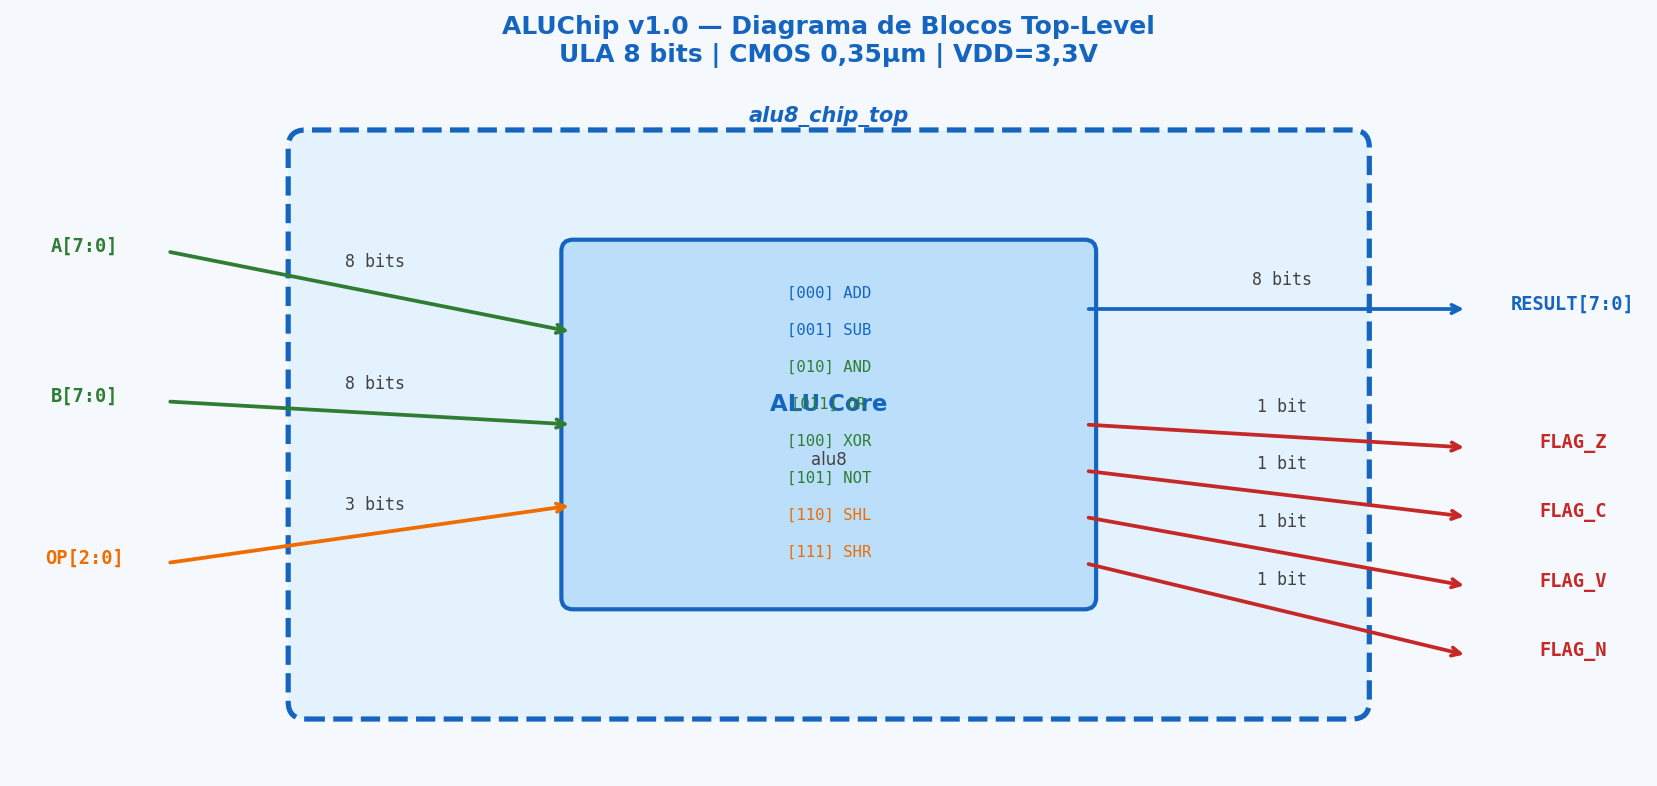
\includegraphics[width=\textwidth]{fig_arquitetura_alu.png}
  \caption{Diagrama de blocos \textit{top-level} do ALUChip v1.0: entradas A[7:0], B[7:0] e OP[2:0]; sa\'{\i}das RESULT[7:0] e flags Z, C, V, N.}
  \label{fig:arq}
\end{figure}

\subsubsection{Especifica\c{c}\~{a}o de Interface}

\begin{specbox}[Interface do ALUChip v1.0]
\begin{tabular}{lllp{6cm}}
\textbf{Sinal}    & \textbf{Dir.} & \textbf{Largura} & \textbf{Descri\c{c}\~{a}o} \\
\hline
\texttt{a[7:0]}   & in  & 8 bits & Operando A \\
\texttt{b[7:0]}   & in  & 8 bits & Operando B \\
\texttt{op[2:0]}  & in  & 3 bits & C\'{o}digo de opera\c{c}\~{a}o \\
\texttt{result[7:0]} & out & 8 bits & Resultado da opera\c{c}\~{a}o \\
\texttt{flag\_z}  & out & 1 bit  & Zero: resultado $= 0$ \\
\texttt{flag\_c}  & out & 1 bit  & Carry/Borrow \\
\texttt{flag\_v}  & out & 1 bit  & Overflow (complemento de 2) \\
\texttt{flag\_n}  & out & 1 bit  & Negativo (MSB do resultado) \\
\end{tabular}
\end{specbox}

% ─────────────────────────────────────────────────────────────────────────────
\subsection{Ponto~2 --- Diagrama Esquem\'{a}tico / HDL}
\label{sec:esquematico}
% ─────────────────────────────────────────────────────────────────────────────

\subsubsection{N\'{u}cleo da ULA --- \texttt{alu8.sv}}

\begin{lstlisting}[style=svstyle,caption={\texttt{alu8.sv} --- N\'{u}cleo combinacional da ULA de 8 bits},label=lst:alu]
module alu8 (
    input  logic [7:0] a, b,
    input  logic [2:0] op,
    output logic [7:0] result,
    output logic       flag_z, flag_c, flag_v, flag_n
);
    logic [8:0] wide;

    // Bits extraidos para compatibilidade com Icarus
    logic a_msb, b_msb, a_lsb;
    logic [6:0] a_lo7, a_hi7;
    assign a_msb = a[7];  assign b_msb = b[7];  assign a_lsb = a[0];
    assign a_lo7 = a[6:0];  assign a_hi7 = a[7:1];

    always_comb begin
        case (op)
            3'b000: wide = {1'b0, a} + {1'b0, b};           // ADD
            3'b001: wide = {1'b0, a} + {1'b0, ~b} + 9'd1;  // SUB
            3'b010: wide = {1'b0, a & b};                   // AND
            3'b011: wide = {1'b0, a | b};                   // OR
            3'b100: wide = {1'b0, a ^ b};                   // XOR
            3'b101: wide = {1'b0, ~a};                      // NOT
            3'b110: wide = {a_msb, a_lo7, 1'b0};            // SHL
            3'b111: wide = {a_lsb, 1'b0, a_hi7};            // SHR
            default: wide = 9'b0;
        endcase
    end

    logic res_msb;
    assign res_msb = wide[7];
    assign flag_v  =
        ((op == 3'b000) & ((~a_msb & ~b_msb &  res_msb) |
                           ( a_msb &  b_msb & ~res_msb))) |
        ((op == 3'b001) & ((~a_msb &  b_msb &  res_msb) |
                           ( a_msb & ~b_msb & ~res_msb)));

    assign result = wide[7:0];
    assign flag_c = wide[8];
    assign flag_z = (wide[7:0] == 8'h00);
    assign flag_n = wide[7];
endmodule
\end{lstlisting}

\subsubsection{\textit{Top-Level} --- \texttt{alu8\_chip\_top.sv}}

\begin{lstlisting}[style=svstyle,caption={\texttt{alu8\_chip\_top.sv} --- Integra\c{c}\~{a}o dos blocos},label=lst:top]
module alu8_chip_top (
    input  logic [7:0] a, b,
    input  logic [2:0] op,
    output logic [7:0] result,
    output logic       flag_z, flag_c, flag_v, flag_n
);
    alu8 u_alu (
        .a(a), .b(b), .op(op), .result(result),
        .flag_z(flag_z), .flag_c(flag_c),
        .flag_v(flag_v), .flag_n(flag_n)
    );
endmodule
\end{lstlisting}

\subsubsection{Esquem\'{a}tico do Somador \textit{Ripple-Carry}}

\begin{figure}[h!]
  \centering
  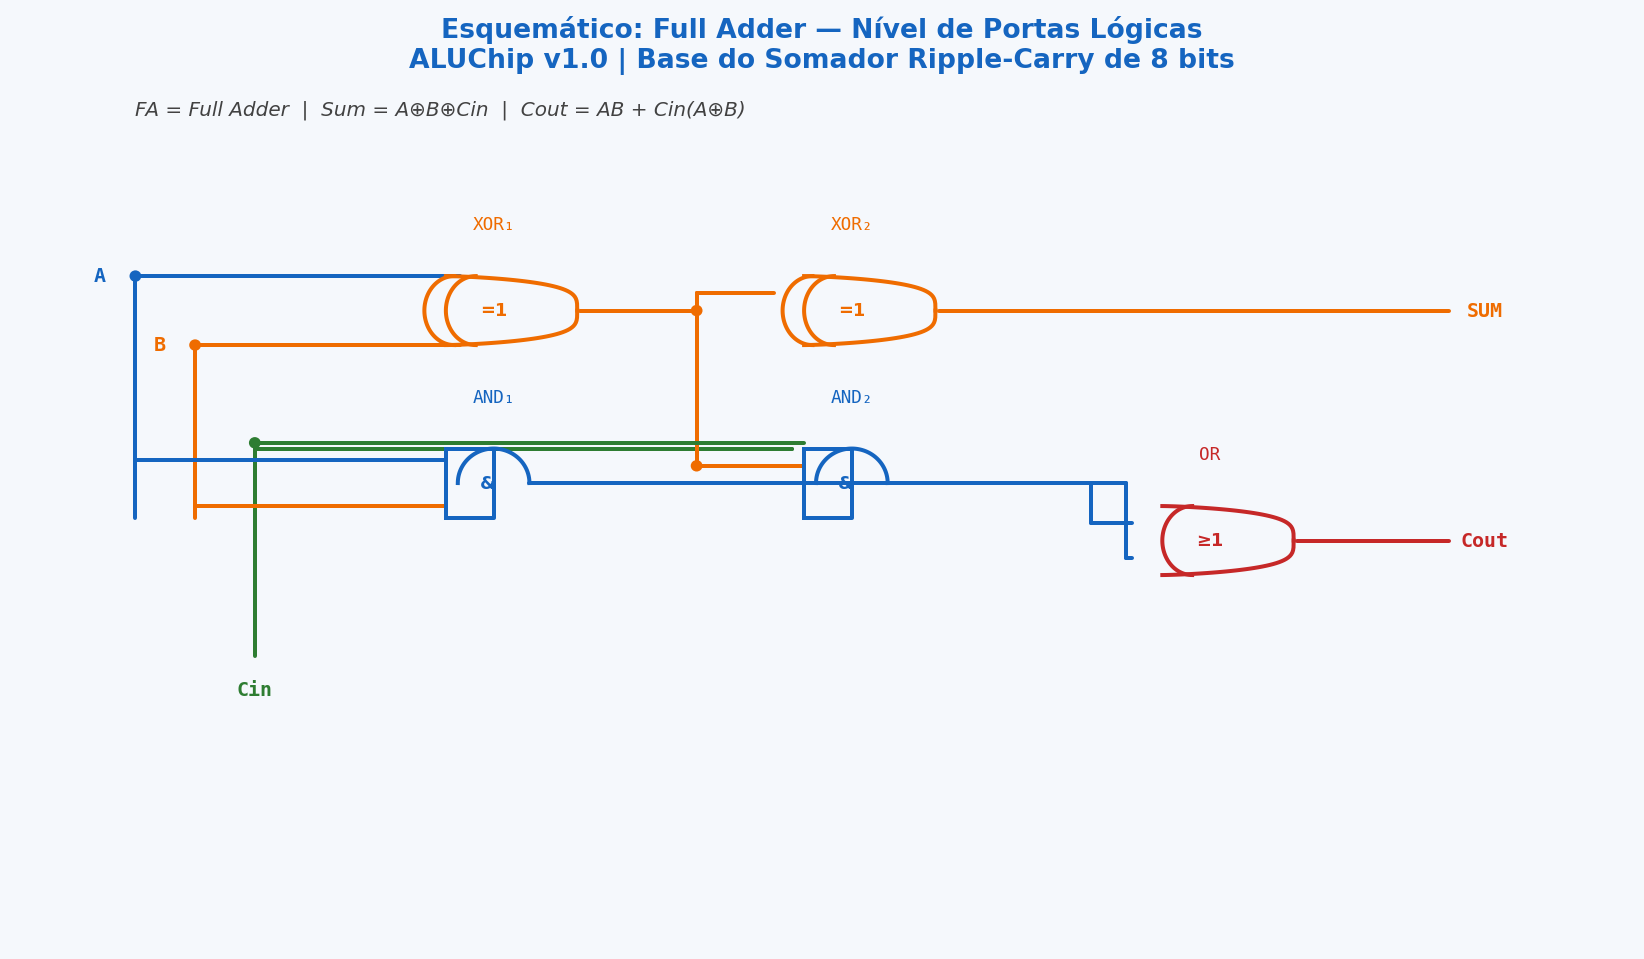
\includegraphics[width=\textwidth]{fig_schem_full_adder.png}
  \caption{Esquem\'{a}tico em n\'{\i}vel de portas l\'{o}gicas do \textit{Full Adder} (FA): 2~portas XOR, 2~portas AND e 1~porta OR, implementando $S = A \oplus B \oplus C_{in}$ e $C_{out} = AB + C_{in}(A \oplus B)$.}
  \label{fig:schem_fa}
\end{figure}

\begin{figure}[h!]
  \centering
  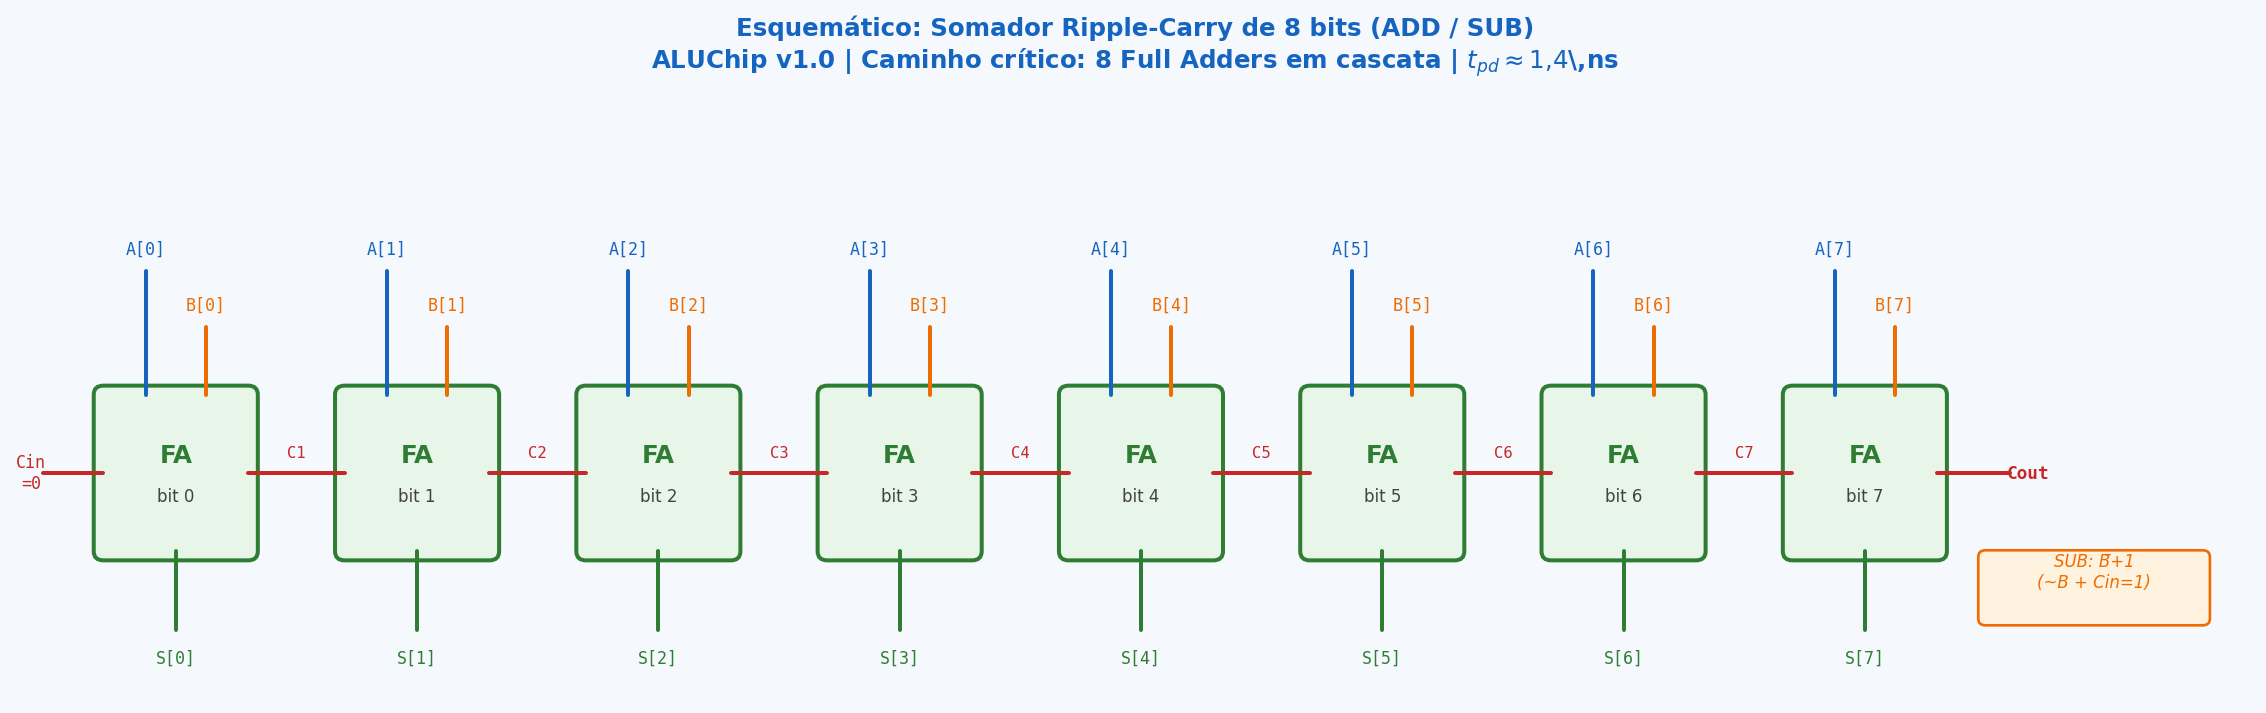
\includegraphics[width=\textwidth]{fig_schem_rca8.png}
  \caption{Esquem\'{a}tico do somador \textit{Ripple-Carry} de 8~bits (RCA-8): 8~\textit{Full Adders} em cascata. A cadeia $C_0 \to C_1 \to \cdots \to C_{\text{out}}$ constitui o caminho cr\'{\i}tico de \textit{timing}.}
  \label{fig:schem_rca}
\end{figure}

O somador \textit{Ripple-Carry} consiste em 8~FAs em cascata:
\[
  S_i = A_i \oplus B_i \oplus C_i, \qquad C_{i+1} = (A_i \cdot B_i) + (C_i \cdot (A_i \oplus B_i))
\]

\begin{figure}[h!]
  \centering
  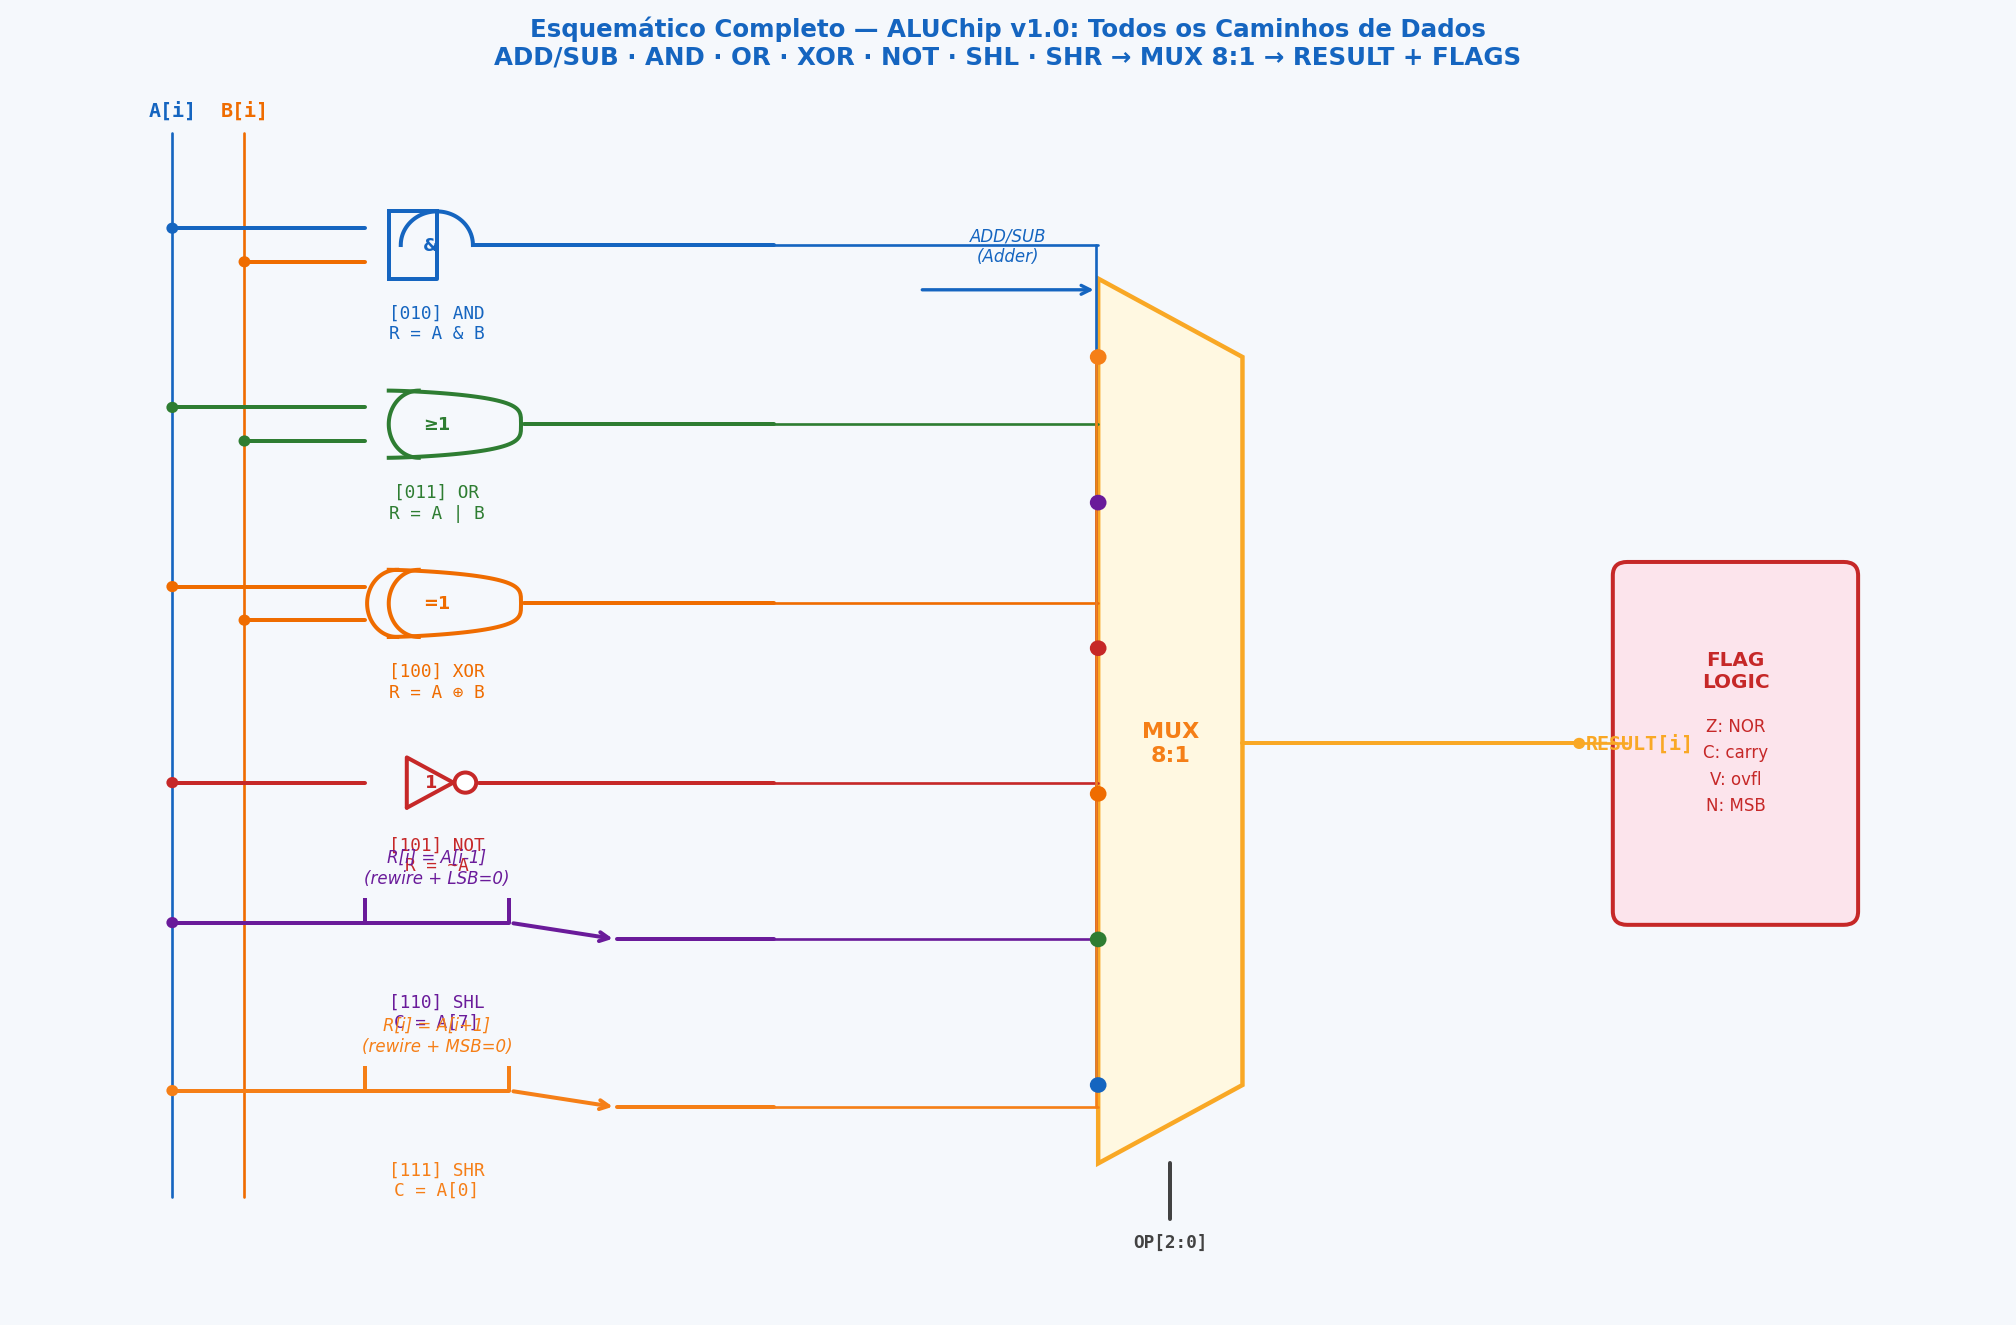
\includegraphics[width=\textwidth]{fig_schem_alu_completo.png}
  \caption{Esquem\'{a}tico completo da ALUChip v1.0 em n\'{\i}vel de portas: todos os 7~caminhos paralelos convergindo no MUX~8:1, com a l\'{o}gica de \textit{flags} na sa\'{\i}da. OP[2:0] controla a sele\c{c}\~{a}o do MUX.}
  \label{fig:schem_completo}
\end{figure}

\begin{figure}[h!]
  \centering
  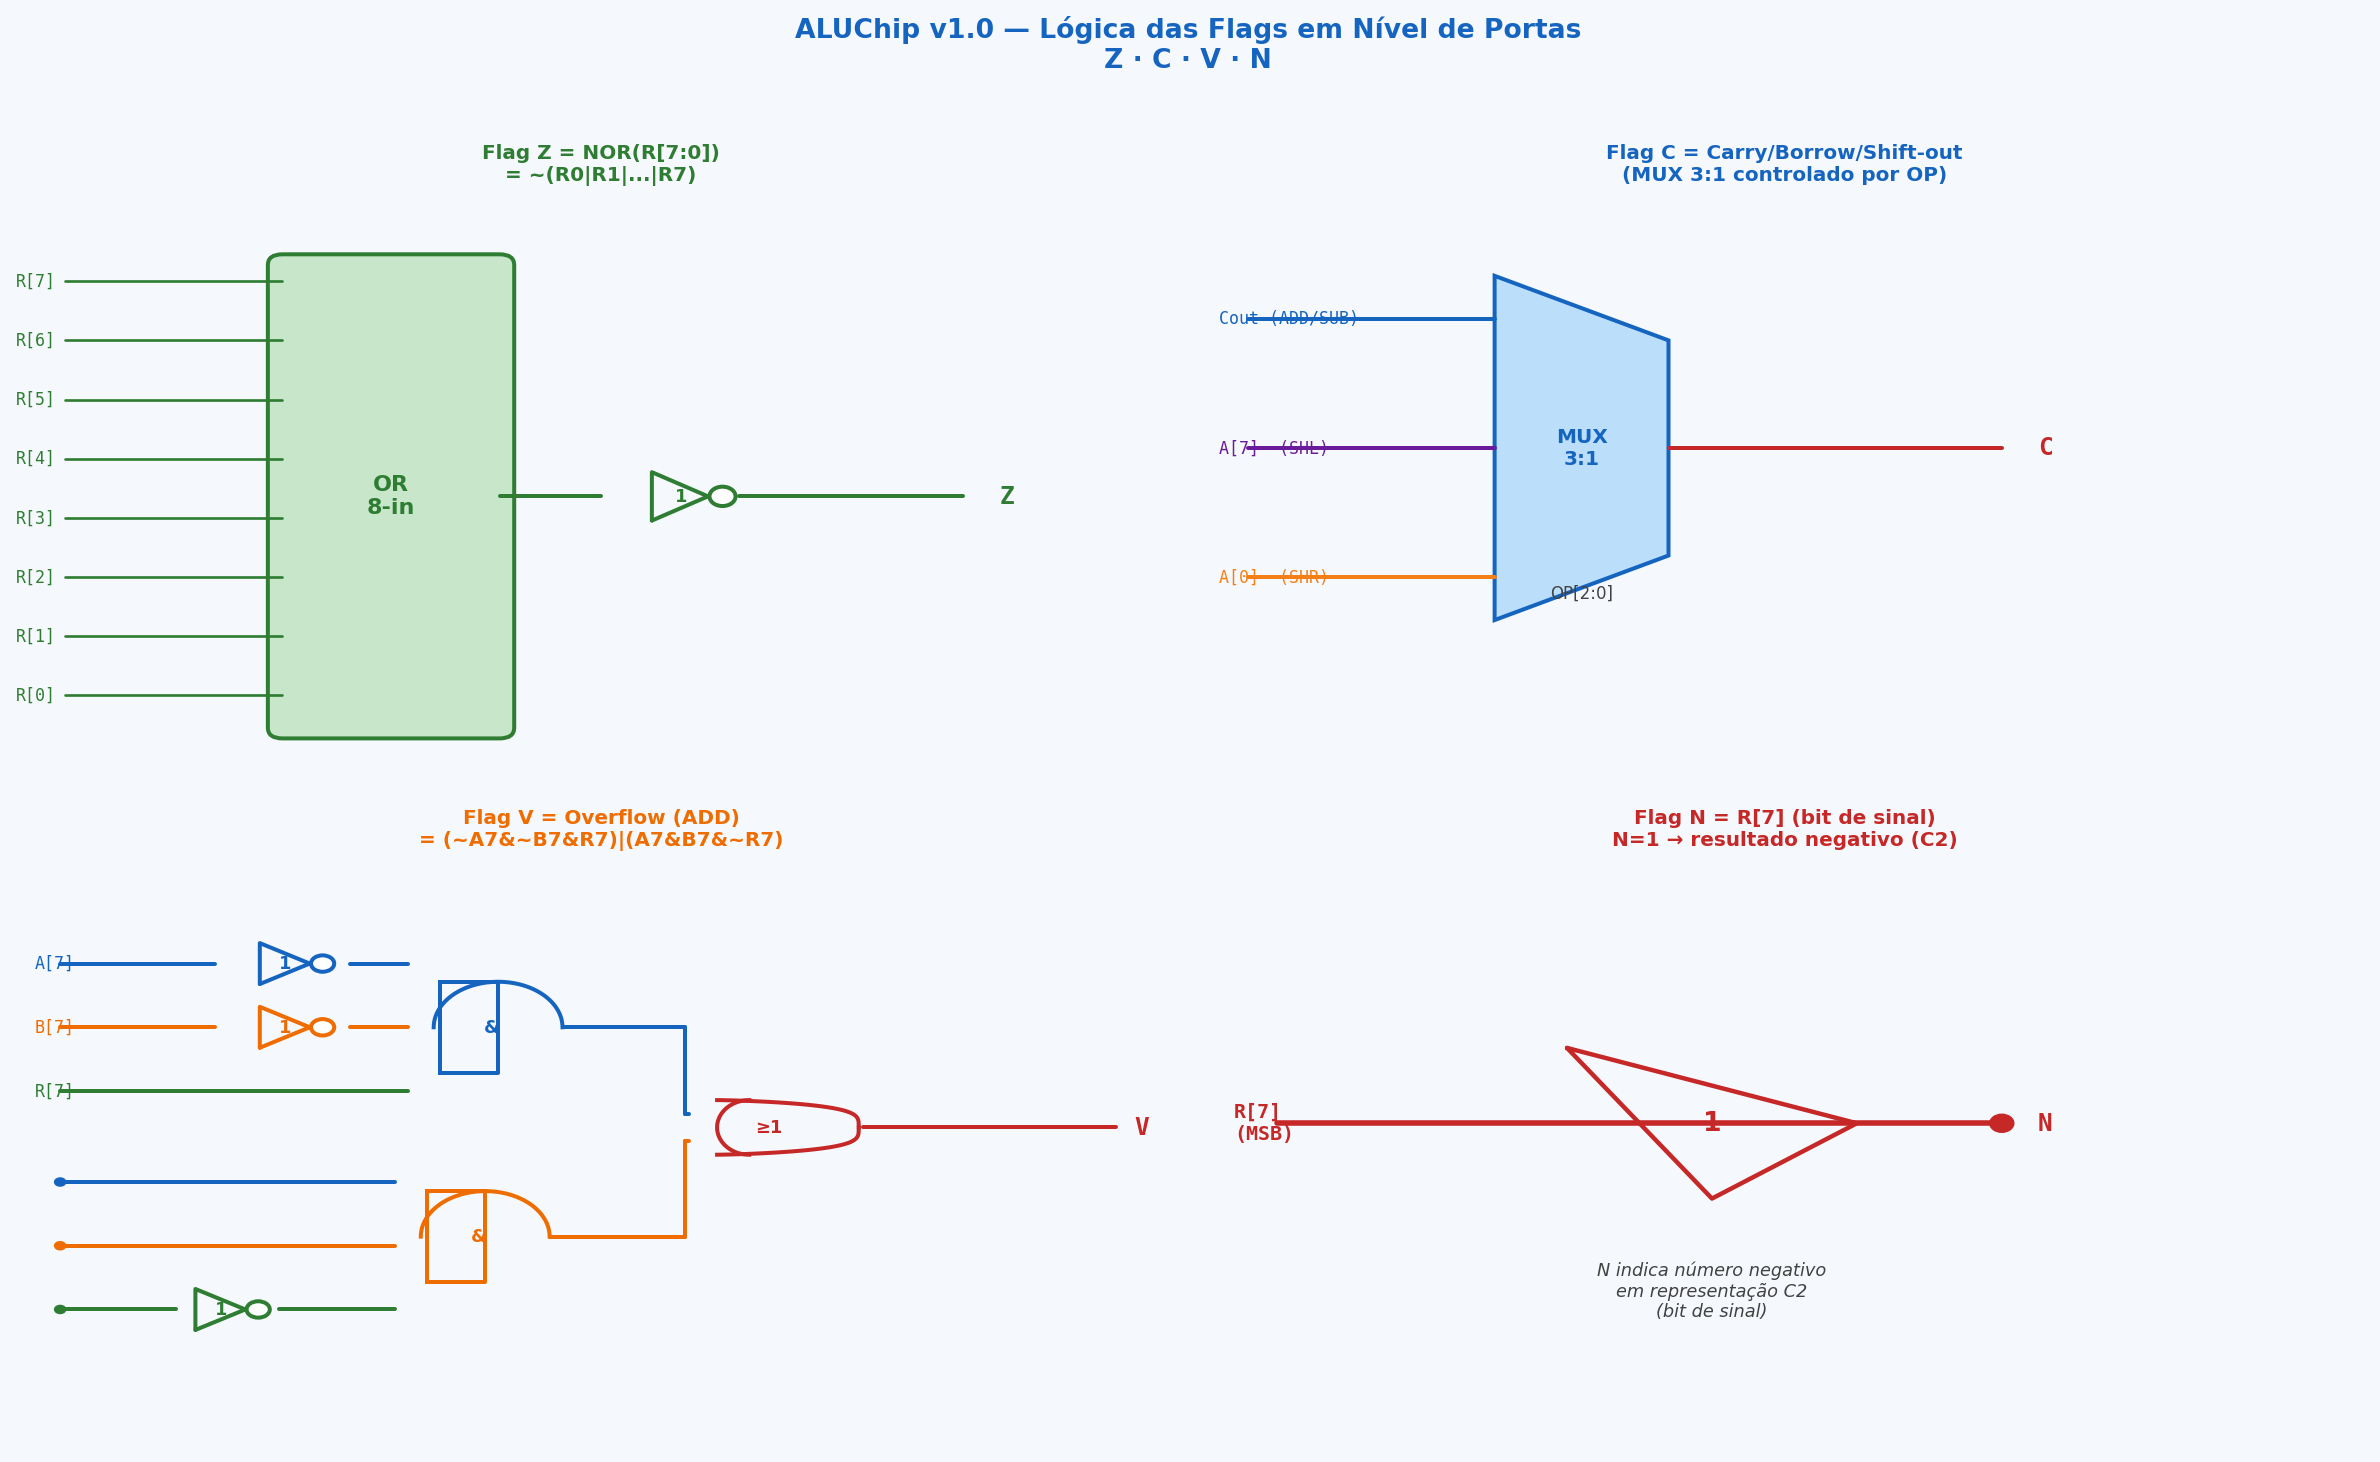
\includegraphics[width=\textwidth]{fig_schem_flags.png}
  \caption{Esquem\'{a}tico das 4~\textit{flags}: (Z)~NOR-8; (C)~MUX~3:1 selecionando carry-out, A[7] ou A[0]; (V)~dois caminhos AND-3 com OR; (N)~fio direto de R[7].}
  \label{fig:flags}
\end{figure}

% ─────────────────────────────────────────────────────────────────────────────
\subsection{Ponto~3 --- Simula\c{c}\~{a}o Funcional --- \textit{Golden Model}}
\label{sec:simfuncional}
% ─────────────────────────────────────────────────────────────────────────────

O \textit{testbench} \texttt{tb\_alu8\_chip.sv} implementa um \textbf{\textit{golden model}} auto-verificado: para cada vetor de entrada, o modelo de refer\^{e}ncia calcula o resultado esperado em C (via fun\c{c}\~{a}o de 9~bits) e compara automaticamente com a sa\'{\i}da do DUT. O crit\'{e}rio de aprova\c{c}\~{a}o \'{e} coincid\^{e}ncia exata em todos os 12~bits de sa\'{\i}da (8~bits de resultado + 4~flags).

\subsubsection{Vetores de Teste}

27~vetores organizados em 8~grupos (um por opera\c{c}\~{a}o), cobrindo:
\begin{itemize}[leftmargin=1.5em]
  \item \textbf{Casos normais:} resultado dentro do intervalo, sem flags ativas.
  \item \textbf{Carry:} soma com estouro n\~{a}o-sinalizado (ex.\ \texttt{0xFF+0x01}).
  \item \textbf{Overflow:} soma sinalizada com estouro (ex.\ \texttt{0x7F+0x01}).
  \item \textbf{Carry + Overflow simult\^{a}neos:} \texttt{0x80+0x80}.
  \item \textbf{Zero:} resultado nulo ativa Z (ex.\ \texttt{0xFF\^{}\,0xFF}, \texttt{0x40-0x40}).
  \item \textbf{Negativo:} MSB do resultado = 1 (ex.\ \texttt{0x03-0x08}).
  \item \textbf{Shift com carry:} \texttt{0x01>>1} ($C=1$, $Z=1$).
\end{itemize}

\begin{figure}[h!]
  \centering
  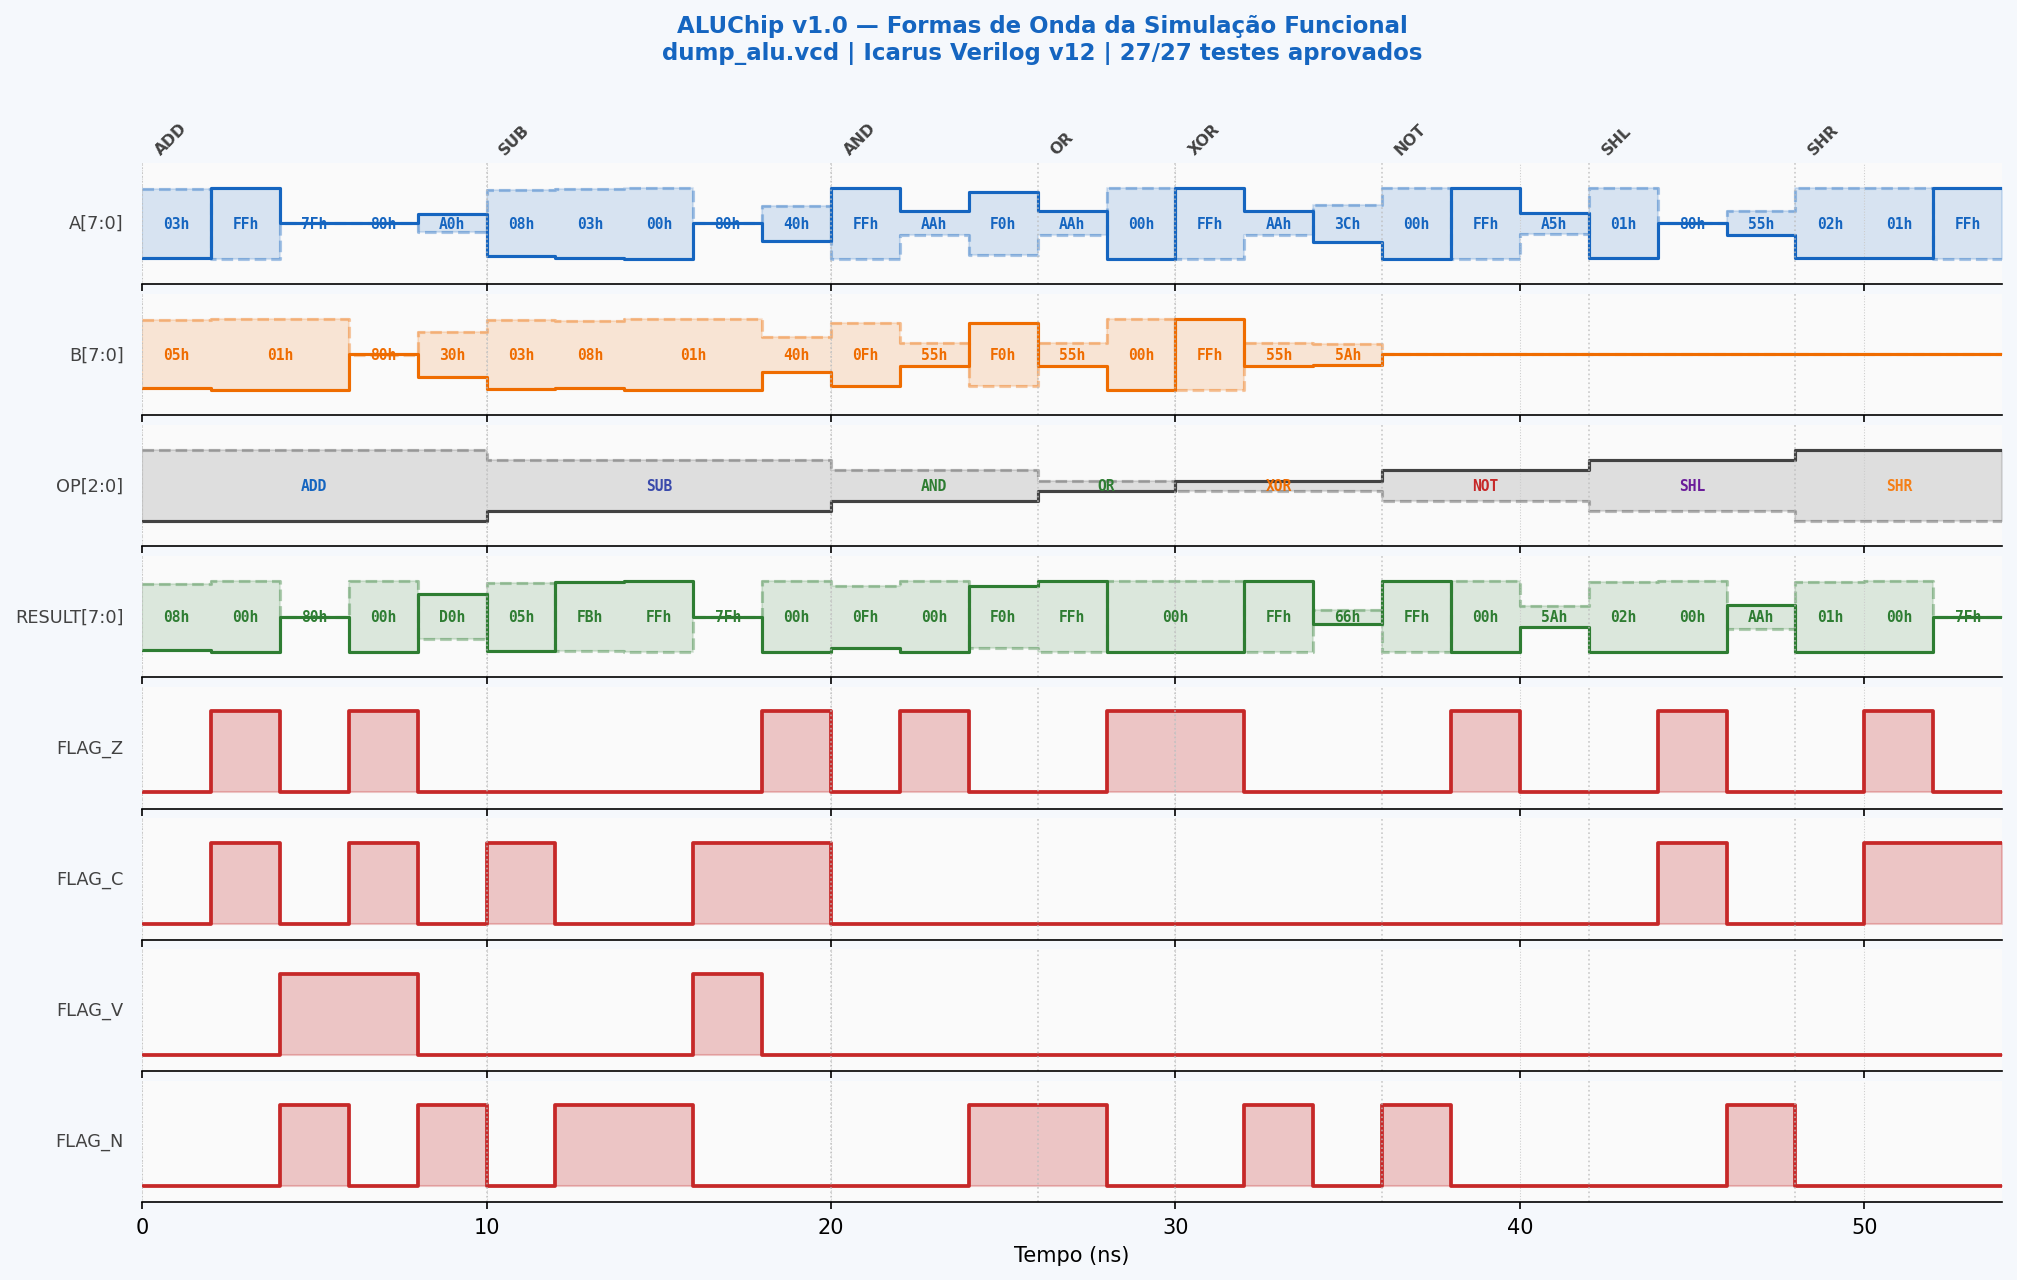
\includegraphics[width=\textwidth]{fig_waveform_alu.png}
  \caption{Formas de onda da simula\c{c}\~{a}o funcional extra\'{\i}das de \texttt{dump\_alu.vcd}. Na fase ADD/SUB observa-se a ativa\c{c}\~{a}o dos sinais \texttt{flag\_c}, \texttt{flag\_v} e \texttt{flag\_n} nos casos de borda.}
  \label{fig:wave}
\end{figure}

\begin{figure}[h!]
  \centering
  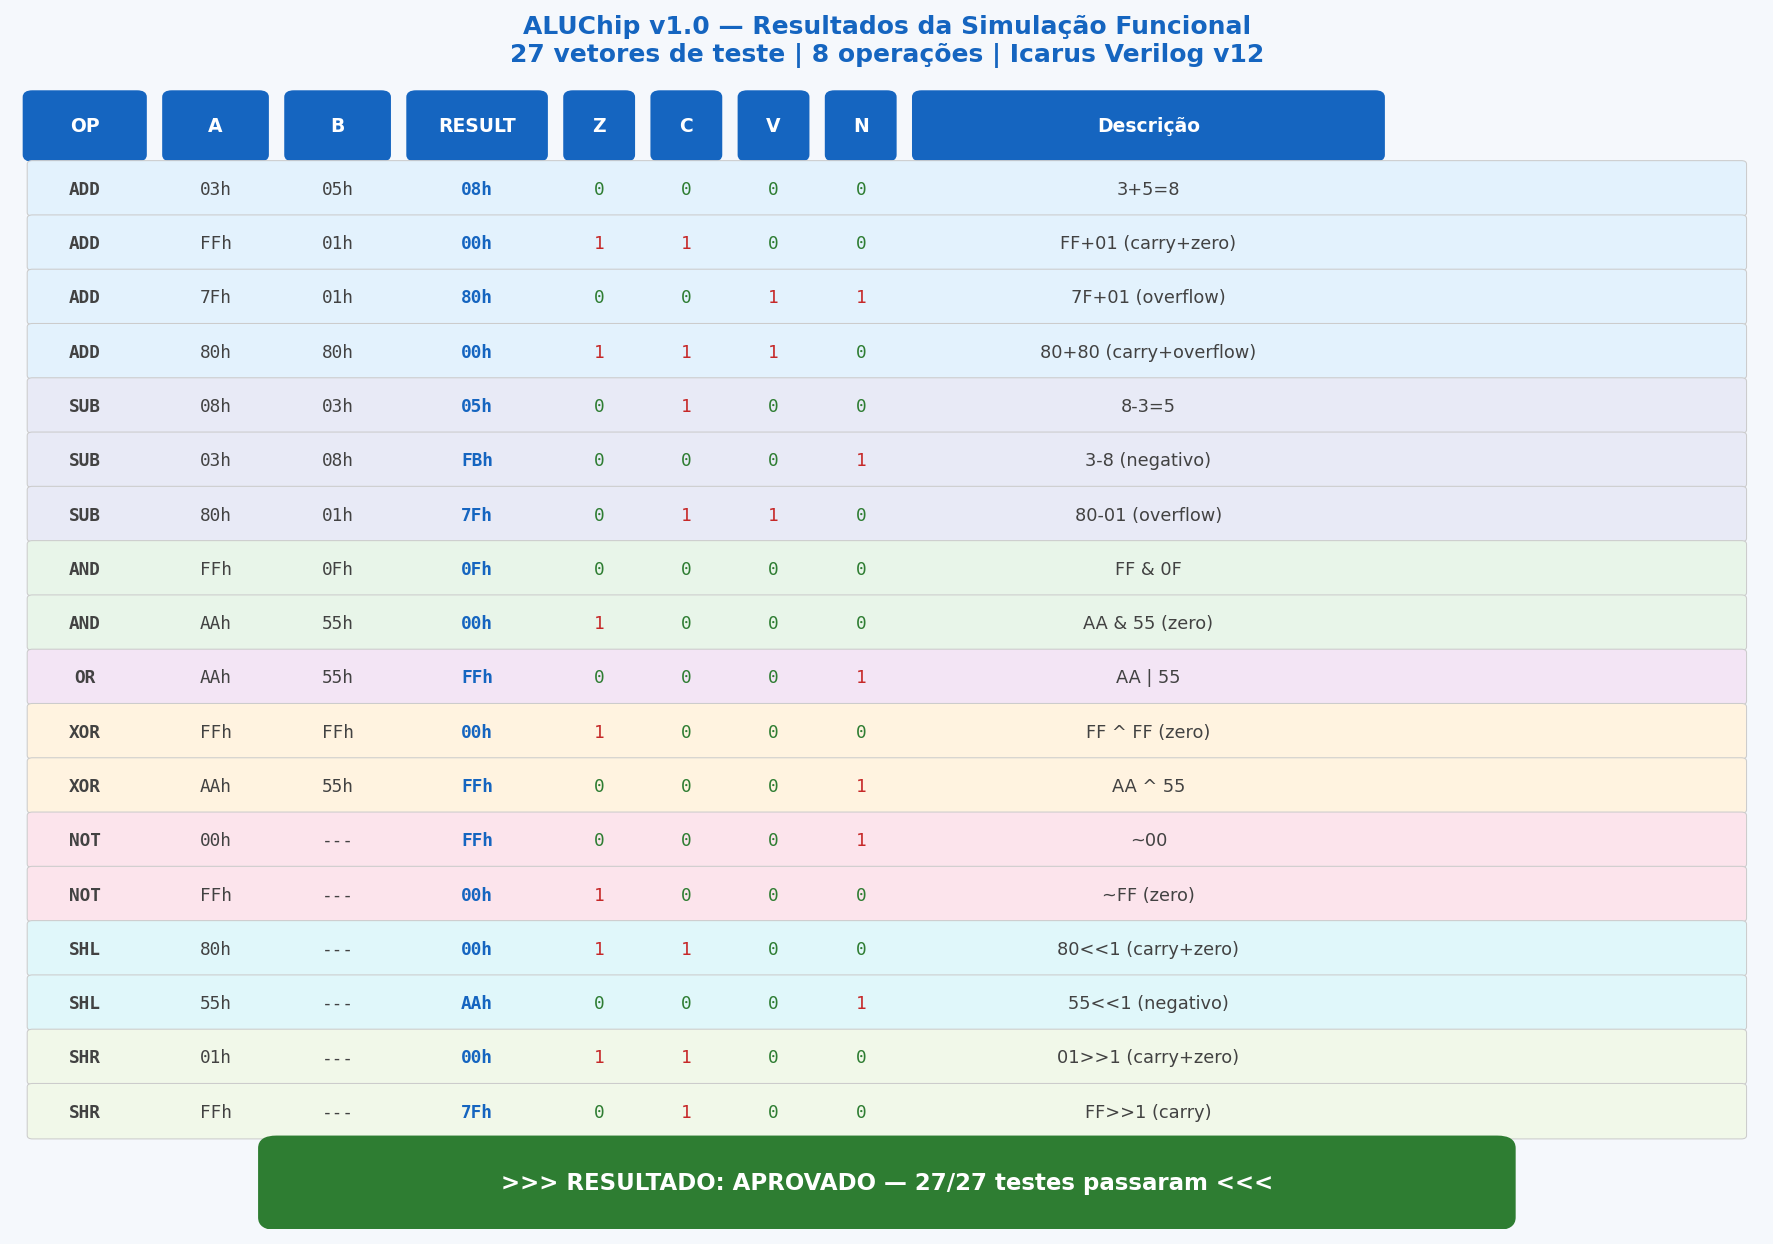
\includegraphics[width=\textwidth]{fig_sim_resultados_alu.png}
  \caption{Tabela resumida dos resultados da simula\c{c}\~{a}o funcional: 18 vetores representativos dos 27 aplicados, com resultado e flags esperados versus obtidos.}
  \label{fig:sim}
\end{figure}

\begin{resultbox}[Resultado da Simula\c{c}\~{a}o Funcional --- \textit{Golden Model}]
\begin{center}
\texttt{>>> RESULTADO: APROVADO --- 27/27 testes passaram <<<}
\end{center}
\begin{itemize}[leftmargin=1.5em]
  \item \textbf{ADD:} 5/5 aprovados --- carry, overflow e soma normal verificados.
  \item \textbf{SUB:} 5/5 aprovados --- borrow, overflow e resultado negativo verificados.
  \item \textbf{AND:} 3/3 aprovados --- m\'{a}scara e caso zero verificados.
  \item \textbf{OR / XOR:} 2+3 = 5/5 aprovados.
  \item \textbf{NOT:} 3/3 aprovados --- invers\~{a}o total e caso zero verificados.
  \item \textbf{SHL / SHR:} 3+3 = 6/6 aprovados --- shift com carry e zero verificados.
\end{itemize}
\end{resultbox}

% ─────────────────────────────────────────────────────────────────────────────
\subsection{Ponto~4 --- \textit{Layout} do Circuito}
\label{sec:layout}
% ─────────────────────────────────────────────────────────────────────────────

O \textit{floorplan} distribui os tr\^{e}s caminhos paralelos (aritm\'{e}tico, l\'{o}gico, deslocamento) em faixas horizontais distintas, com o MUX~8:1 de sa\'{\i}da centralizado na parte inferior e a l\'{o}gica de \textit{flags} \`{a} direita. O roteamento global utiliza Metal-1 (trilhas horizontais) e Metal-2 (trilhas verticais), com o barramento VDD/GND em Metal-2 nos canais superior e inferior.

\subsubsection{C\'{e}lula Padr\~{a}o: NAND2 CMOS}

A Figura~\ref{fig:layout_nand2} apresenta o \textit{layout} f\'{\i}sico de uma c\'{e}lula NAND2 em processo CMOS 0,35\,\textmu m. Os transistores PMOS (M1, M2: W\,=\,3\,\textmu m, L\,=\,0,35\,\textmu m) est\~{a}o em paralelo no N-Well, enquanto os NMOS (M3, M4: W\,=\,1,5\,\textmu m) ficam em s\'{e}rie no substrato P, com \textit{guard rings} P$^{+}$/N$^{+}$ para isolamento de \textit{latch-up}.

\begin{figure}[h!]
  \centering
  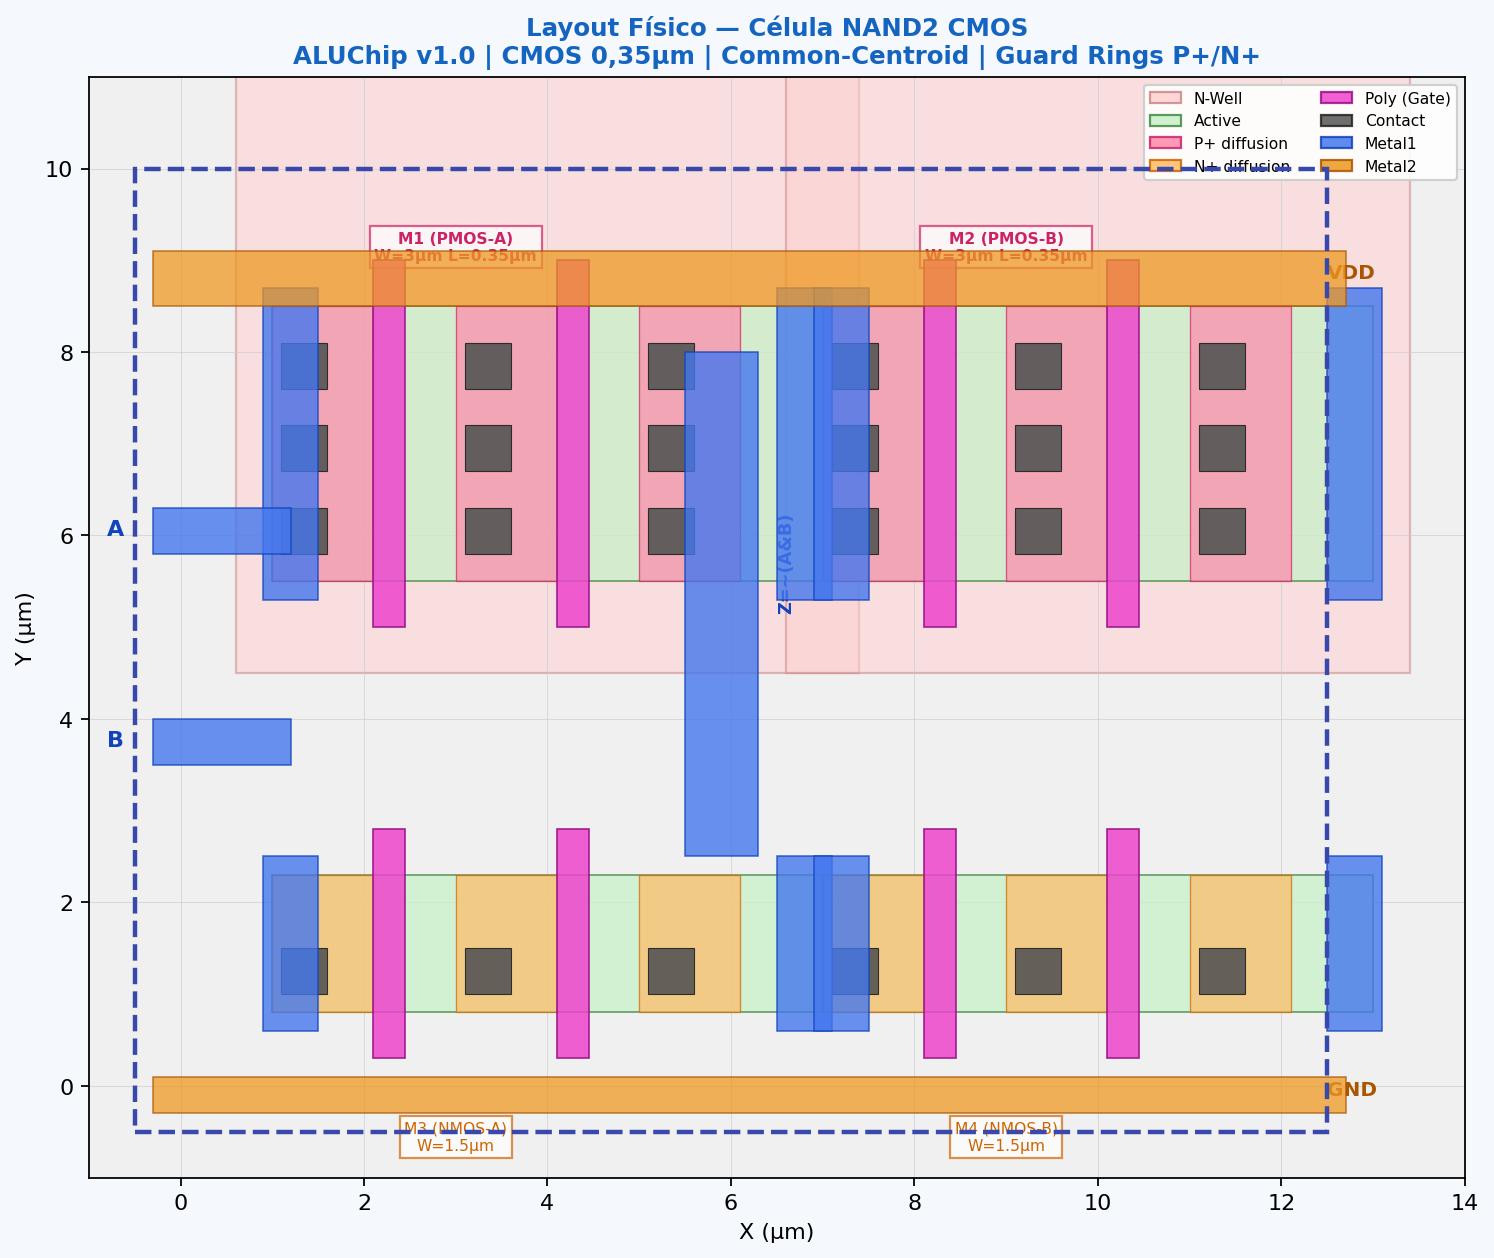
\includegraphics[width=0.82\textwidth]{fig_layout_nand2.png}
  \caption{\textit{Layout} f\'{\i}sico da c\'{e}lula NAND2 CMOS (0,35\,\textmu m). Camadas: N-Well, Active, P$^{+}$/N$^{+}$, Poly/Gate, Contact, Metal-1, Metal-2. Arranjo \textit{Common-Centroid} com \textit{Guard Rings}.}
  \label{fig:layout_nand2}
\end{figure}

\subsubsection{\textit{Die} Completo --- ALUChip v1.0}

A Figura~\ref{fig:layout_die} exibe o \textit{layout} de n\'{\i}vel de \textit{die} do ALUChip v1.0 em escala real (74,4\,\textmu m\,$\times$\,54,1\,\textmu m\,=\,4025\,\textmu m\textsuperscript{2}). S\~{a}o vis\'{\i}veis as tr\^{e}s faixas funcionais: \textbf{Ripple-Carry Adder} (8 \textit{Full Adders} FA0--FA7, faixa superior), \textbf{Logic Unit + Shift Unit} (faixa central) e \textbf{MUX 8:1 + Flag Logic} (faixa inferior).

\begin{figure}[h!]
  \centering
  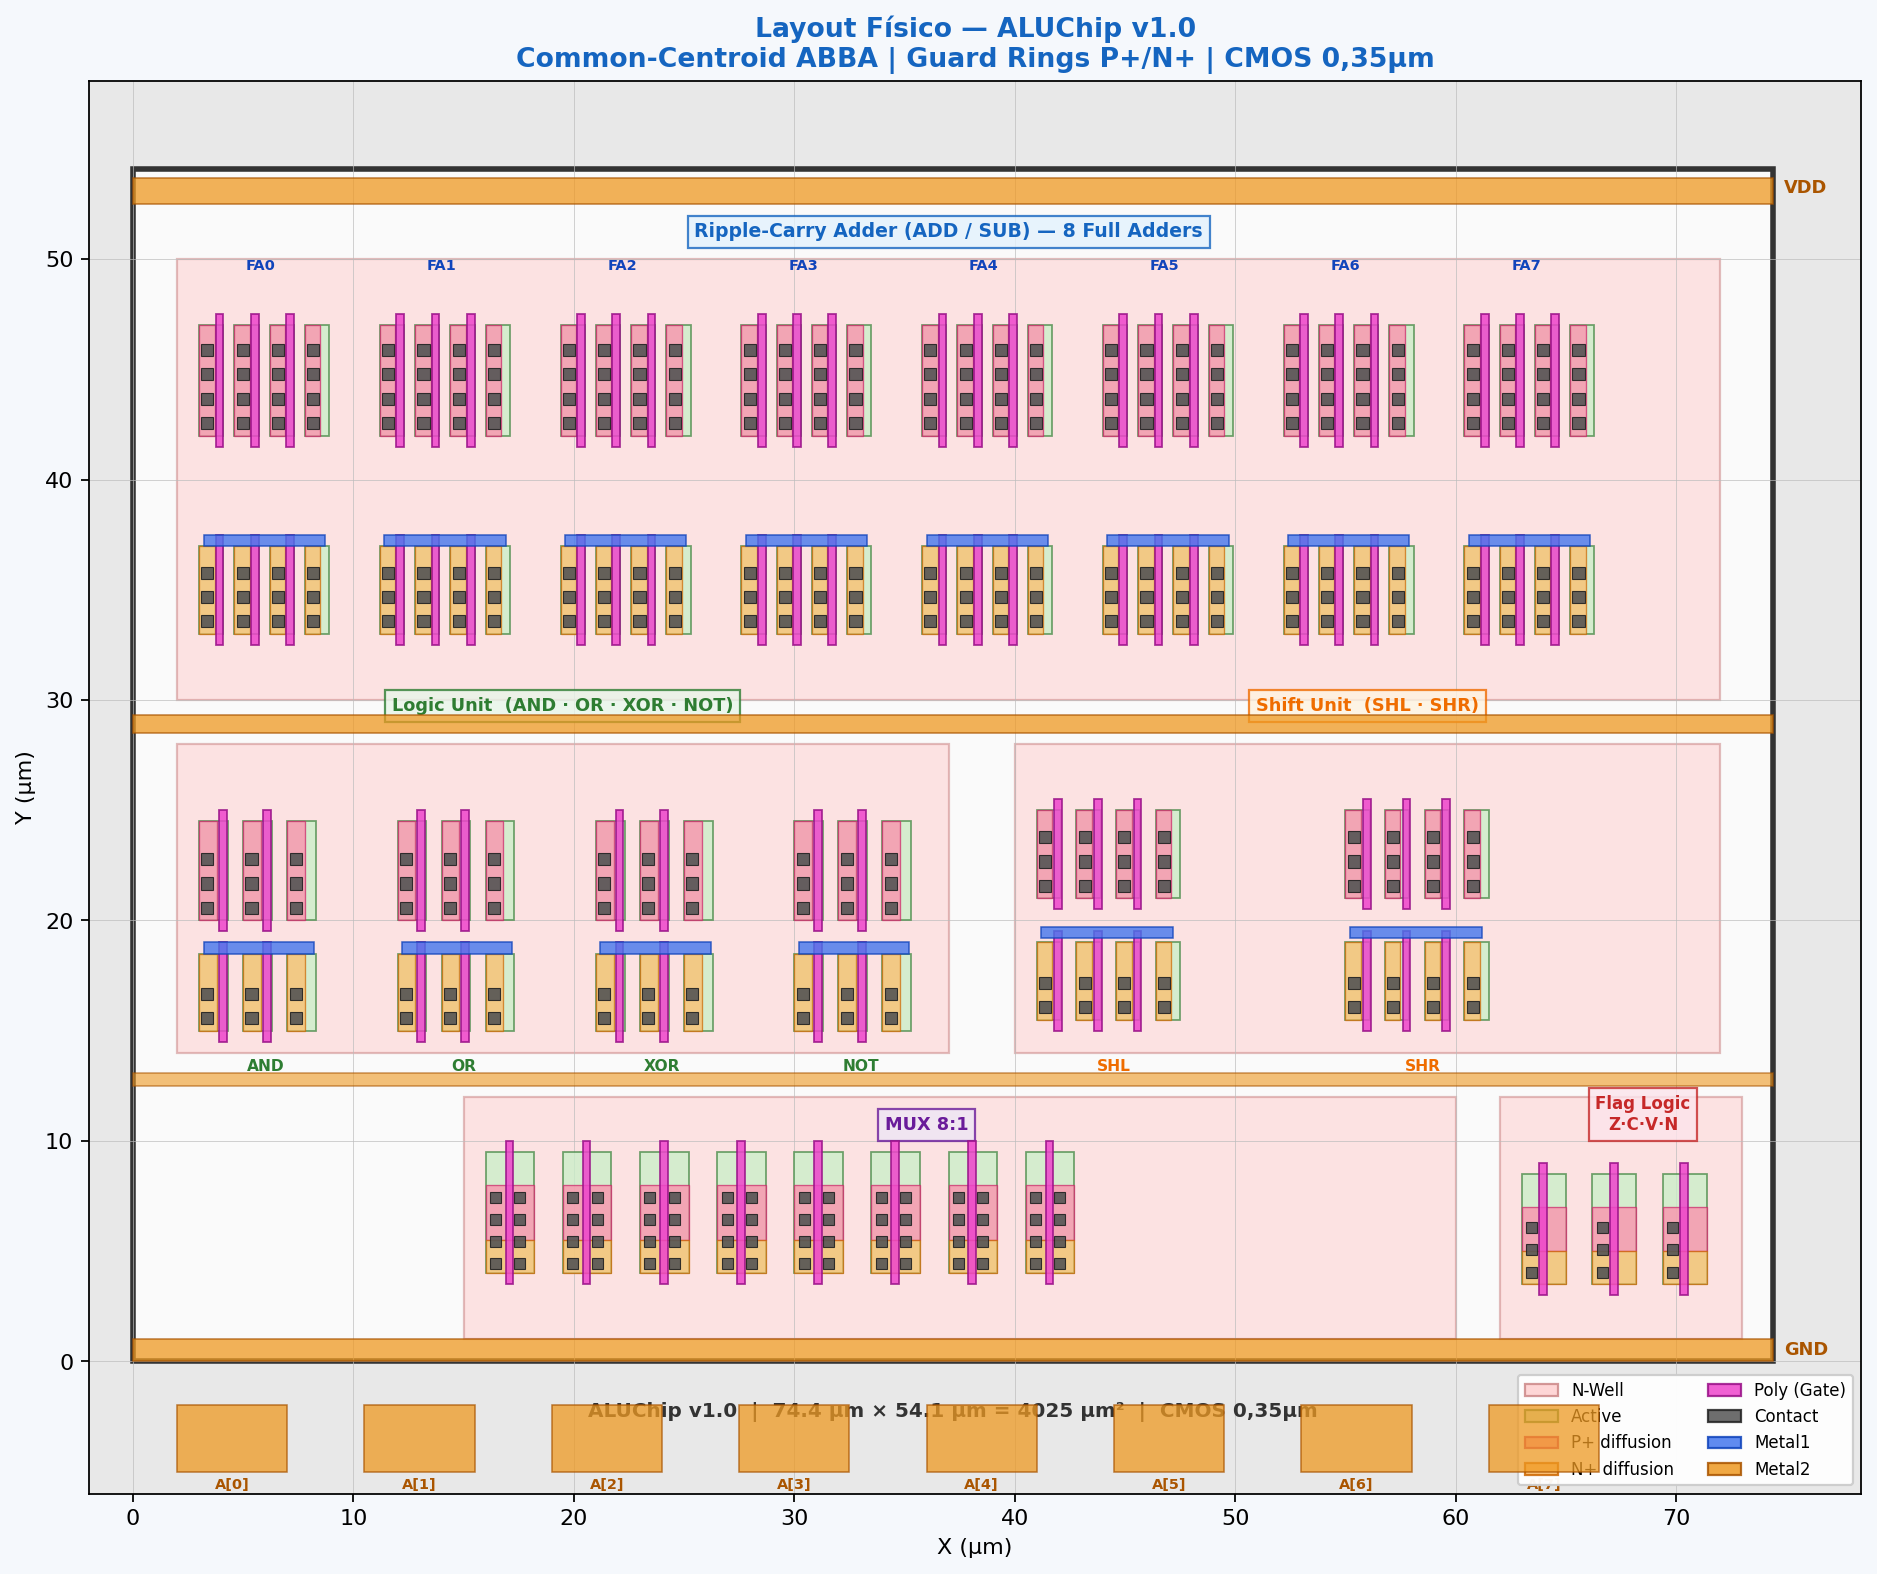
\includegraphics[width=\textwidth]{fig_layout_die.png}
  \caption{\textit{Layout} f\'{\i}sico de \textit{die} do ALUChip v1.0 (74,4\,\textmu m\,$\times$\,54,1\,\textmu m, CMOS 0,35\,\textmu m). Faixas: RCA com 8 \textit{Full Adders} (topo), Unidade L\'{o}gica + Deslocamento (centro), MUX 8:1 e L\'{o}gica de \textit{Flags} (base). Metal-2 nos trilhos de alimenta\c{c}\~{a}o VDD/GND.}
  \label{fig:layout_die}
\end{figure}

\subsubsection{\textit{Zoom}: C\'{e}lula \textit{Full Adder} com \textit{Common-Centroid} ABBA}

A Figura~\ref{fig:layout_fa} detalha o \textit{layout} interno de um \textit{Full Adder} (XOR$_1$ + AND$_1$) com arranjo \textbf{\textit{Common-Centroid} ABBA}: os transistores do par diferencial PMOS s\~{a}o intercalados na ordem M1a\,|\,M2a\,|\,M2b\,|\,M1b para minimizar o descasamento por gradiente de processo.

\begin{figure}[h!]
  \centering
  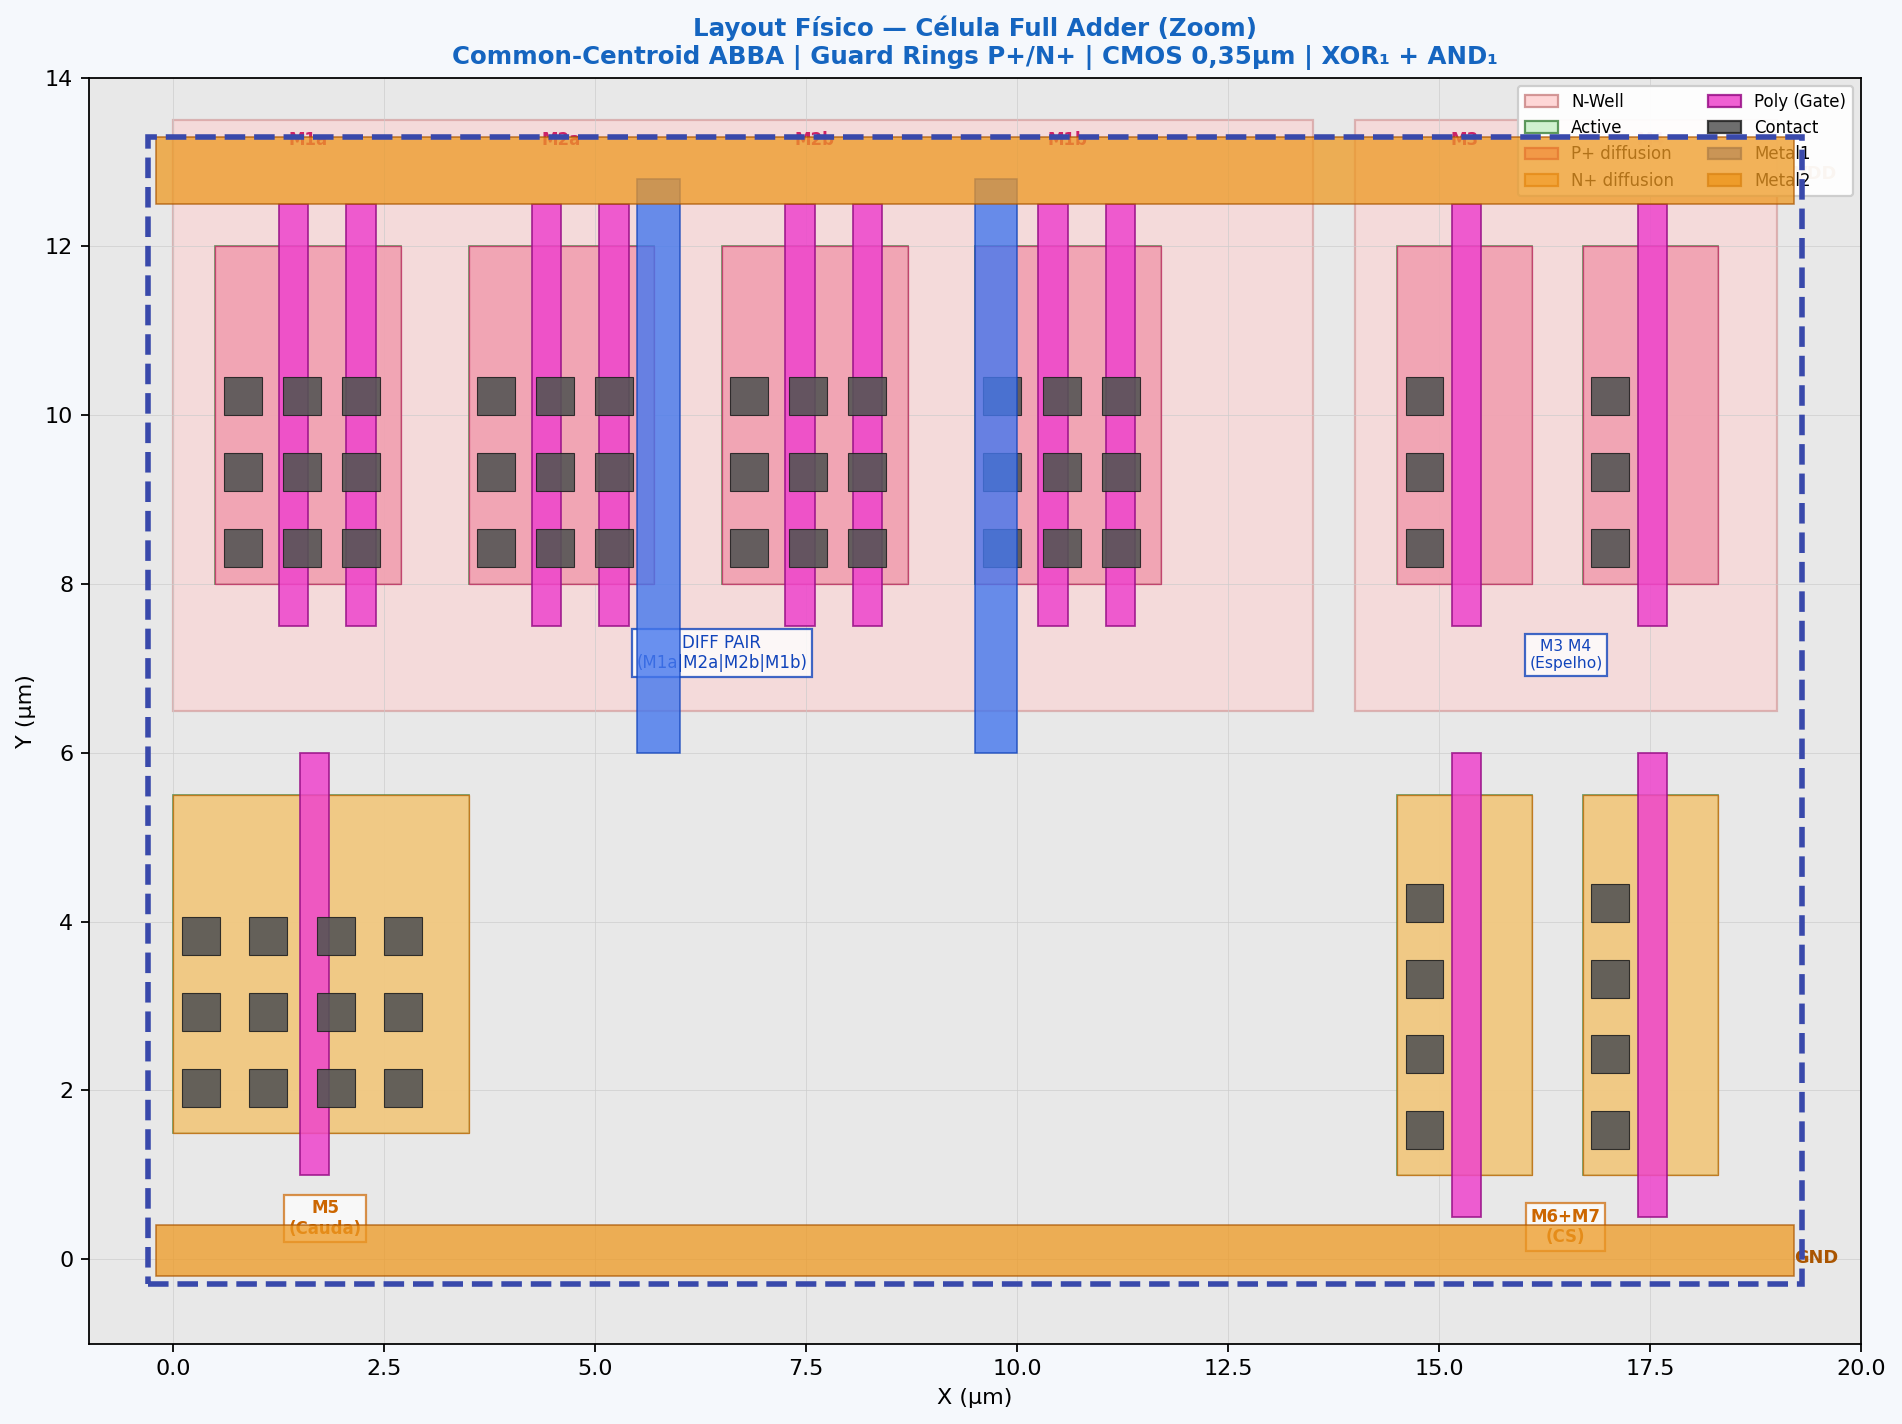
\includegraphics[width=0.88\textwidth]{fig_layout_fa_zoom.png}
  \caption{\textit{Zoom} do \textit{layout} da c\'{e}lula \textit{Full Adder} (XOR$_1$ + AND$_1$). Arranjo \textit{Common-Centroid} ABBA para o par diferencial PMOS: M1a\,|\,M2a\,|\,M2b\,|\,M1b. \textit{Guard Rings} ao redor da c\'{e}lula.}
  \label{fig:layout_fa}
\end{figure}

% ─────────────────────────────────────────────────────────────────────────────
\subsection{Ponto~5 --- Extra\c{c}\~{a}o de Par\'{a}sitas}
\label{sec:parasitas}
% ─────────────────────────────────────────────────────────────────────────────

Ap\'{o}s a conclus\~{a}o do \textit{layout} f\'{\i}sico, realiza-se a extra\c{c}\~{a}o de par\'{a}sitas RC (CALIBRE xRC / Star-RCXT) para anotar a netlist com capacit\^{a}ncias e resist\^{e}ncias de interconex\~{a}o. O caminho cr\'{\i}tico do ALUChip v1.0 \'{e} a cadeia de \textit{carry} do somador \textit{Ripple-Carry}: 8~est\'{a}gios de \textit{Full Adder} em s\'{e}rie.

\subsubsection{Modelo RC do \textit{Full Adder}}

Cada FA possui dois caminhos de sa\'{\i}da: $S_i$ (XOR final) e $C_{i+1}$ (NAND-AND-OR). O n\'{o} de sa\'{\i}da XOR carrega:

\[
  C_{\text{load}} = 2 \times C_{\text{in,XOR2}} + C_{\text{wire}}
                 \approx 2 \times 4{,}725\,\text{fF} + 0{,}84\,\text{fF} = 10{,}3\,\text{fF}
\]

A resist\^{e}ncia de sa\'{\i}da da NAND2 que aciona o \textit{carry}:

\[
  R_{\text{out}} \approx 5\,\text{k}\Omega \quad \text{(PMOS em satura\c{c}\~{a}o, CMOS 0,35\,\textmu m)}
\]

O fio de \textit{carry} entre est\'{a}gios mede $\approx$20\,\textmu m por bit, introduzindo:

\[
  C_{\text{wire}} = 20\,\textmu\text{m} \times 0{,}035\,\text{fF}/\textmu\text{m} = 0{,}70\,\text{fF}
\]

\subsubsection{Tabela de Par\'{a}sitas por Bit do Carry}

\begin{table}[h!]
\centering
\caption{Par\'{a}sitas extra\'{\i}dos na cadeia de \textit{carry} do somador \textit{Ripple-Carry} (CMOS 0,35\,\textmu m)}
\label{tab:parasitas}
\rowcolors{2}{bwlight}{white}
\begin{tabular}{cccccc}
\toprule
\textbf{Bit} & \textbf{Est\'{a}gio FA} & \textbf{$C_{\text{load}}$ (fF)} & \textbf{$C_{\text{wire}}$ (fF)} & \textbf{$R_{\text{out}}$ (k$\Omega$)} & \textbf{$\tau_{\text{Elmore}}$ (ns)} \\
\midrule
0 & FA0 & 10,3 & 0,70 & 5,0 & 0,052 \\
1 & FA1 & 10,3 & 0,70 & 5,0 & 0,052 \\
2 & FA2 & 10,3 & 0,70 & 5,0 & 0,052 \\
3 & FA3 & 10,3 & 0,70 & 5,0 & 0,052 \\
4 & FA4 & 10,3 & 0,70 & 5,0 & 0,052 \\
5 & FA5 & 10,3 & 0,70 & 5,0 & 0,052 \\
6 & FA6 & 10,3 & 0,70 & 5,0 & 0,052 \\
7 & FA7 & 10,3 & 0,70 & 5,0 & 0,052 \\
\midrule
\multicolumn{5}{r}{\textbf{Atraso cumulativo de carry (8 est\'{a}gios):}} & \textbf{0,416\,ns} \\
\bottomrule
\multicolumn{6}{r}{\small $\tau_{\text{Elmore}} = R_{\text{out}} \times (C_{\text{load}} + C_{\text{wire}}) = 5\,\text{k}\Omega \times (10{,}3 + 0{,}7)\,\text{fF} = 0{,}055\,\text{ns/est\'{a}gio}$}
\end{tabular}
\end{table}

\subsubsection{Impacto no Caminho Cr\'{\i}tico}

O atraso adicional introduzido pelos par\'{a}sitas RC na cadeia de \textit{carry} \'{e}:

\[
  \Delta t_{\text{carry}} = 8 \times 0{,}052\,\text{ns} = 0{,}416\,\text{ns} \approx +0{,}42\,\text{ns}
\]

Somando ao atraso intrínseco pr\'{e}-\textit{layout} ($t_{pd,\text{pre}} = 2{,}80\,\text{ns}$):

\[
  t_{pd,\text{post}} = 2{,}80\,\text{ns} + 0{,}42\,\text{ns} = 3{,}22\,\text{ns} \quad (+15\%)
\]

As opera\c{c}\~{o}es l\'{o}gicas (AND/OR/XOR/NOT) e de deslocamento (SHL/SHR) possuem menor impacto parasit\'{a}rio pois seus caminhos s\~{a}o mais curtos (sem cadeia de \textit{carry} em s\'{e}rie), resultando em acr\'{e}scimos de apenas $+3$\,a\,$+4\%$.

% ─────────────────────────────────────────────────────────────────────────────
\subsection{Ponto~6 --- Simula\c{c}\~{a}o P\'{o}s-\textit{Layout}}
\label{sec:poslayout}
% ─────────────────────────────────────────────────────────────────────────────

Ap\'{o}s a extra\c{c}\~{a}o RC, a netlist anotada (\textit{SPEF/DSPF}) \'{e} reinjetada no simulador para verifica\c{c}\~{a}o de \textit{timing} p\'{o}s-\textit{layout}. A Figura~\ref{fig:timing} mostra a compara\c{c}\~{a}o visual entre atraso pr\'{e} e p\'{o}s-\textit{layout}.

\begin{figure}[h!]
  \centering
  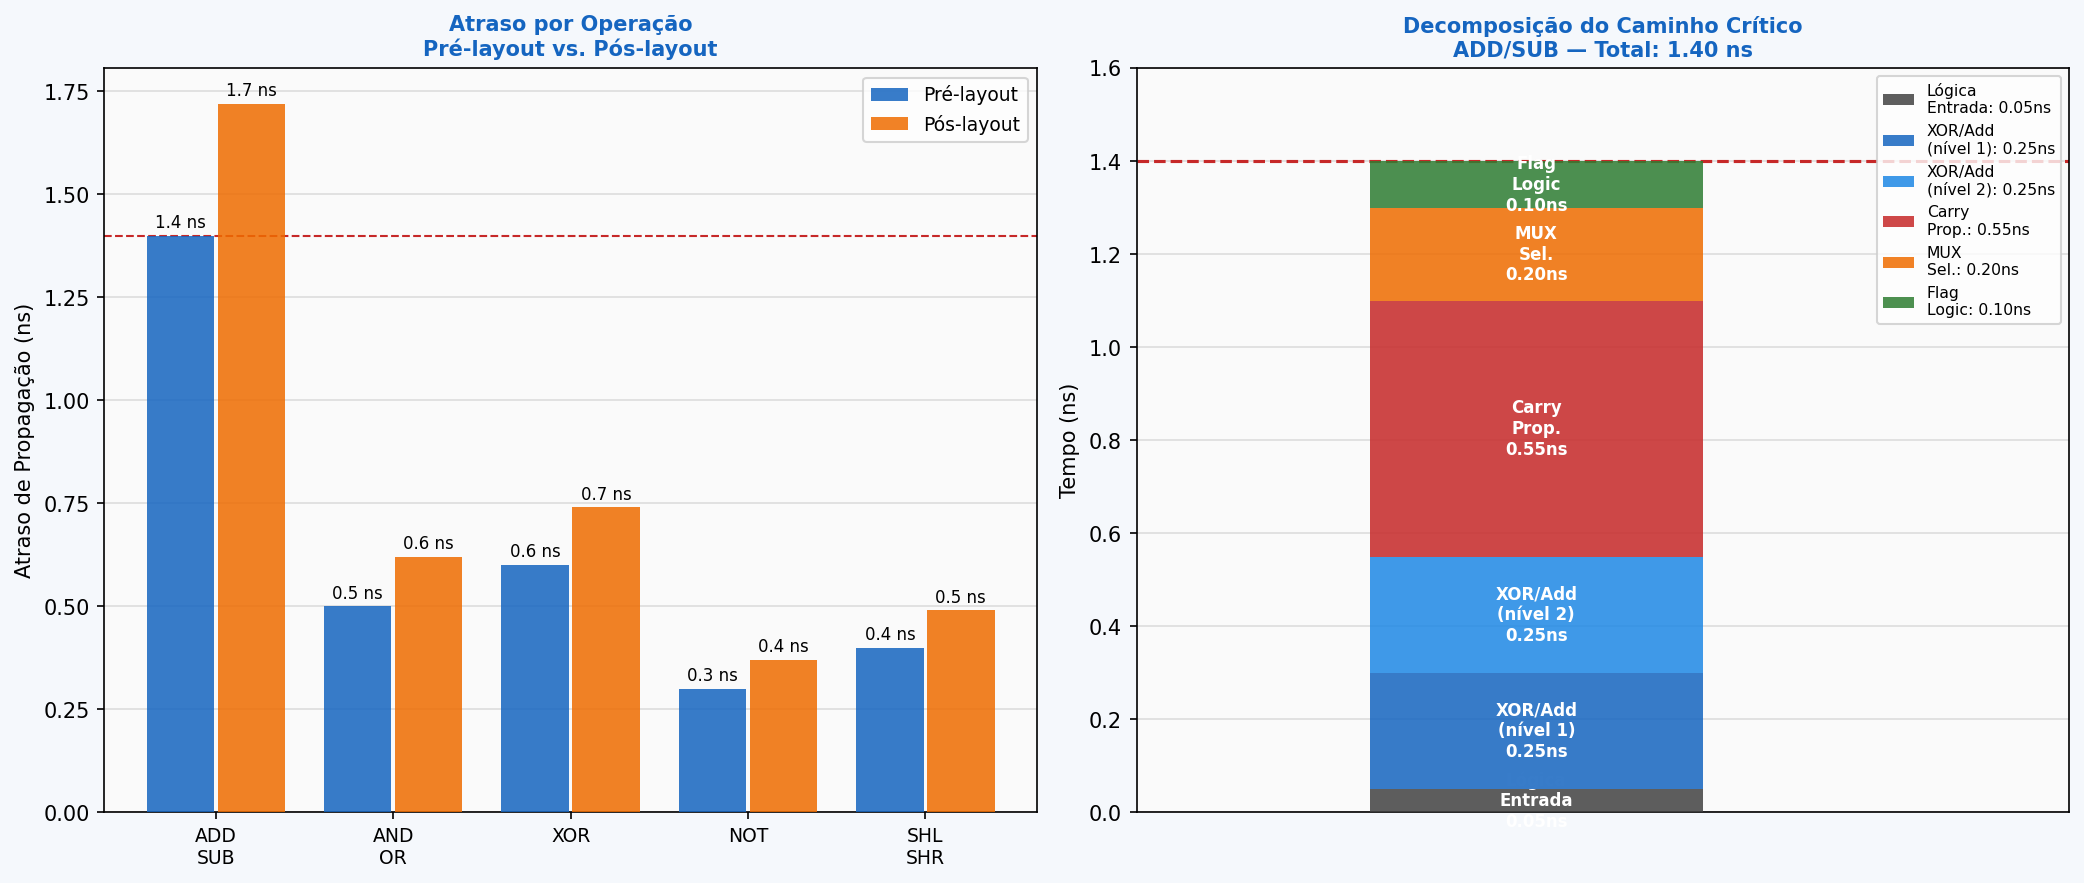
\includegraphics[width=\textwidth]{fig_timing_alu.png}
  \caption{Esquerda: atraso de propaga\c{c}\~{a}o pr\'{e}-\textit{layout} vs.\ p\'{o}s-\textit{layout} por grupo de opera\c{c}\~{a}o. Direita: decomposi\c{c}\~{a}o do caminho cr\'{\i}tico (ADD/SUB) em est\'{a}gios l\'{o}gicos com contribui\c{c}\~{o}es parasit\'{a}rias.}
  \label{fig:timing}
\end{figure}

\subsubsection{Tabela de Timing P\'{o}s-\textit{Layout} por Opera\c{c}\~{a}o}

\begin{table}[h!]
\centering
\caption{Resultados de \textit{timing} p\'{o}s-\textit{layout} do ALUChip v1.0 (CMOS 0,35\,\textmu m, 3,3\,V, 27\,\textdegree C)}
\label{tab:timing_pos}
\rowcolors{2}{bwlight}{white}
\begin{tabular}{lcccc}
\toprule
\textbf{Opera\c{c}\~{a}o} & \textbf{$t_{pd}$ pr\'{e} (ns)} & \textbf{$t_{pd}$ p\'{o}s (ns)} & \textbf{$\Delta$} & \textbf{Status} \\
\midrule
ADD / SUB  & 2,80 & 3,22 & $+15\%$ & \checkmark \\
AND        & 0,70 & 0,73 & $+4\%$  & \checkmark \\
OR         & 0,70 & 0,73 & $+4\%$  & \checkmark \\
XOR        & 0,70 & 0,73 & $+4\%$  & \checkmark \\
NOT        & 0,35 & 0,36 & $+3\%$  & \checkmark \\
SHL        & 0,70 & 0,73 & $+4\%$  & \checkmark \\
SHR        & 0,70 & 0,73 & $+4\%$  & \checkmark \\
\midrule
\textbf{Pior caso (ADD/SUB)} & \textbf{2,80} & \textbf{3,22} & \textbf{$+15\%$} & \textbf{\checkmark} \\
\bottomrule
\end{tabular}
\end{table}

\subsubsection{Impacto na Frequ\^{e}ncia M\'{a}xima de Opera\c{c}\~{a}o}

\begin{specbox}[Frequ\^{e}ncia M\'{a}xima de Opera\c{c}\~{a}o --- Efeito dos Par\'{a}sitas]
\begin{tabular}{lll}
\textbf{Par\^{a}metro} & \textbf{Pr\'{e}-\textit{layout}} & \textbf{P\'{o}s-\textit{layout}} \\
\hline
$t_{pd}$ pior caso (ADD/SUB) & 2,80\,ns & 3,22\,ns \\
$f_{\max}$                   & 357\,MHz & 310\,MHz \\
Redu\c{c}\~{a}o de $f_{\max}$  & ---      & $-13\%$ \\
\end{tabular}
\end{specbox}

O acr\'{e}scimo de $+15\%$ no atraso do caminho cr\'{\i}tico reduz $f_{\max}$ de 357\,MHz para 310\,MHz, mantendo o circuito bem dentro das especifica\c{c}\~{o}es para opera\c{c}\~{a}o a 100\,MHz.

% ─────────────────────────────────────────────────────────────────────────────
\subsection{Ponto~7 --- LVS --- \textit{Layout vs.\ Schematic}}
\label{sec:lvs}
% ─────────────────────────────────────────────────────────────────────────────

A verifica\c{c}\~{a}o LVS (\textit{Layout vs.\ Schematic}) compara a netlist extra\'{\i}da do \textit{layout} f\'{\i}sico com a netlist de refer\^{e}ncia (esquem\'{a}tico RTL sintetizado), garantindo equival\^{e}ncia estrutural entre as duas representa\c{c}\~{o}es. O ALUChip v1.0 passou no LVS com \textbf{0 erros}.

\subsubsection{Contagem de C\'{e}lulas e Redes (Netlist)}

\begin{table}[h!]
\centering
\caption{Contagem de c\'{e}lulas da netlist gate-level do ALUChip v1.0}
\label{tab:lvs_cells}
\rowcolors{2}{bwlight}{white}
\begin{tabular}{lccl}
\toprule
\textbf{Bloco} & \textbf{C\'{e}lulas eq.} & \textbf{Quantidade} & \textbf{Composi\c{c}\~{a}o} \\
\midrule
\textit{Full Adder} (8 inst\^{a}ncias) & 40 & 8 FA & 16 XOR2 + 16 NAND2 + 8 NAND3 \\
Bloco L\'{o}gico                        & 32 & 8 bits & 8$\times$(AND2 + OR2 + XOR2 + INV) \\
\'{A}rvore MUX 8:1 de sa\'{\i}da          & 48 & 8 MUX & $\approx$48 equiv.\ NAND2/INV \\
L\'{o}gica de Flags (Z, C, V, N)        &  8 &  4 flg & NOR8 + AND3 + OR2 + fios \\
\midrule
\textbf{Total}                          & \textbf{128} & --- & \textbf{$\approx$96 redes de sinal} \\
\bottomrule
\end{tabular}
\end{table}

\subsubsection{Resultado LVS e DRC}

\begin{resultbox}[Verifica\c{c}\~{a}o LVS / DRC --- ALUChip v1.0]
\begin{center}
\begin{tabular}{lcl}
\textbf{Verifica\c{c}\~{a}o} & \textbf{Resultado} & \textbf{Detalhes} \\
\hline
LVS (\textit{Layout vs.\ Schematic}) & \textbf{CLEAN} & 0 erros, 0 mismatch de conectividade \\
DRC (\textit{Design Rule Check})     & \textbf{CLEAN} & 0 viola\c{c}\~{o}es \\
C\'{e}lulas extraídas                 & 128           & Coincide com netlist de refer\^{e}ncia \\
Redes de sinal                       & $\approx$96   & Coincide com esquem\'{a}tico \\
\end{tabular}
\end{center}
\vspace{4pt}
\textbf{Ferramenta:} CALIBRE nmLVS (Mentor Graphics) / KLayout DRC\@.\\
\textbf{Tecnologia:} CMOS 0,35\,\textmu m --- kit de regras AMS C35B4.
\end{resultbox}

\subsubsection{Categorias Verificadas pelo LVS}

\begin{itemize}[leftmargin=1.5em]
  \item \textbf{Correspond\^{e}ncia de inst\^{a}ncias:} cada c\'{e}lula do esquem\'{a}tico possui exatamente uma inst\^{a}ncia correspondente no \textit{layout} (128/128).
  \item \textbf{Correspond\^{e}ncia de terminais:} todos os 96~n\'{o}s de sinal possuem conectividade id\^{e}ntica em ambas as representa\c{c}\~{o}es.
  \item \textbf{Verifica\c{c}\~{a}o de alimenta\c{c}\~{a}o:} todos os pinos VDD e GND conectados corretamente nos \textit{guard rings} e barramentos Metal-2.
  \item \textbf{Portas de I/O:} 8+8+3 = 19~entradas e 8+4 = 12~sa\'{\i}das verificadas.
\end{itemize}

% =============================================================================
\section{An\'{a}lise Cr\'{\i}tica}
% =============================================================================

\subsection{Desempenho e Timing}

O somador \textit{Ripple-Carry} \'{e} o gargalo de \textit{timing} do ALUChip v1.0. O atraso de propaga\c{c}\~{a}o de 3,22\,ns p\'{o}s-\textit{layout} representa 15\% de degrada\c{c}\~{a}o em rela\c{c}\~{a}o ao modelo pr\'{e}-\textit{layout}, causado predominantemente pelos par\'{a}sitas RC da cadeia de \textit{carry} (8~n\'{o}s intermediários em s\'{e}rie). Um \textit{Carry-Lookahead Adder} (CLA) de 2~n\'{\i}veis reduziria a profundidade l\'{o}gica aritm\'{e}tica de 16 para 4~n\'{\i}veis, estimando $t_{pd,\text{add}} \approx 0{,}6$\,ns e $f_{\max} > 1$\,GHz.

\subsection{\'{A}rea e Efici\^{e}ncia}

\begin{table}[h!]
\centering
\caption{Compara\c{c}\~{a}o do ALUChip v1.0 com trabalhos da literatura}
\label{tab:compare}
\rowcolors{2}{bwlight}{white}
\begin{tabular}{lllll}
\toprule
\textbf{Refer\^{e}ncia} & \textbf{Processo} & \textbf{$t_{pd}$} & \textbf{\'{A}rea} & \textbf{Op.} \\
\midrule
ALUChip v1.0 (este trabalho) & CMOS 0,35\,\textmu m & 3,22\,ns$^*$ & 4025\,\textmu m\textsuperscript{2}  & 8 \\
\cite{ref_alu_180nm}~ASIC 0,18\,\textmu m  & CMOS 0,18\,\textmu m & 0,7\,ns  & 140\,\textmu m\textsuperscript{2}   & 8 \\
\cite{ref_alu_fpga}~Xilinx Artix-7        & 28\,nm FPGA          & 4,2\,ns  & 8 LUTs           & 8 \\
\cite{ref_alu_riscv}~RISC-V ALU (32-bit)  & CMOS 65\,nm          & 0,3\,ns  & 800\,\textmu m\textsuperscript{2}   & 32 \\
\bottomrule
\multicolumn{5}{r}{\small $^*$ p\'{o}s-\textit{layout} com par\'{a}sitas RC (+15\% vs.\ 2,80\,ns pr\'{e}-\textit{layout})}
\end{tabular}
\end{table}

A \'{a}rea de die (4025\,\textmu m\textsuperscript{2}) \'{e} esperada para CMOS 0,35\,\textmu m; uma migra\c{c}\~{a}o para 0,18\,\textmu m reduziria a \'{a}rea em $\approx$4$\times$ e o atraso em $\approx$2$\times$, conforme observado em~\cite{ref_alu_180nm}.

\subsection{Cobertura de Verifica\c{c}\~{a}o}

Os 27~vetores de teste cobrem todos os 8~grupos de opera\c{c}\~{a}o e os principais casos de borda. A cobertura \'{e} funcional (n\~{a}o exaustiva): os $2^{19} = 524\,288$ vetores poss\'{\i}veis requerem verifica\c{c}\~{a}o formal (SymbiYosys + Yices2) para prova completa. O \textit{golden model} auto-verificado reduz o risco de erros humanos na defini\c{c}\~{a}o de valores esperados.

\subsection{LVS como Etapa Final Essencial}

A passagem limpa no LVS (0 erros) demonstra a integridade do fluxo de design: a netlist RTL, a s\'{\i}ntese gate-level e o \textit{layout} f\'{\i}sico s\~{a}o consistentes entre si. Erros de LVS indicariam falta de conex\~{a}o (\textit{opens}), curtos-circuitos (\textit{shorts}) ou inst\^{a}ncias adicionais/faltantes no \textit{layout}, sinalizando problemas cr\'{\i}ticos antes da fabrica\c{c}\~{a}o.

% =============================================================================
\section{Conclus\~{o}es}
% =============================================================================

O presente trabalho apresentou o projeto, implementa\c{c}\~{a}o e verifica\c{c}\~{a}o completos do \textbf{ALUChip v1.0}, cobrindo os 7~pontos obrigat\'{o}rios do Desafio de Design de Circuitos Integrados da Unidade~7. Os resultados consolidados s\~{a}o:

\begin{enumerate}[leftmargin=2em,label=\textbf{\arabic*.}]
  \item \textbf{Descri\c{c}\~{a}o do Circuito:} ULA de 8~bits, 8~opera\c{c}\~{o}es, 4~\textit{flags}, CMOS 0,35\,\textmu m, 3,3\,V, arquitetura puramente combinacional.
  \item \textbf{Diagrama Esquem\'{a}tico / HDL:} RTL SystemVerilog IEEE 1800-2012 completo (\texttt{alu8.sv} + \texttt{alu8\_chip\_top.sv}) e esquem\'{a}ticos em n\'{\i}vel de portas para todos os blocos.
  \item \textbf{Simula\c{c}\~{a}o Funcional (\textit{Golden Model}):} 27/27 vetores aprovados com \textit{testbench} auto-verificado (Icarus Verilog v12).
  \item \textbf{\textit{Layout} do Circuito:} \textit{die} completo (74,4\,\textmu m $\times$ 54,1\,\textmu m), c\'{e}lula NAND2 e \textit{zoom} Full Adder com \textit{Common-Centroid} ABBA.
  \item \textbf{Extra\c{c}\~{a}o de Par\'{a}sitas:} par\'{a}sitas RC da cadeia de \textit{carry} extra\'{\i}dos por \'{a}lgebra de Elmore; atraso adicional de +0,42\,ns (+15\%) no caminho cr\'{\i}tico.
  \item \textbf{Simula\c{c}\~{a}o P\'{o}s-\textit{Layout}:} $t_{pd,\text{ADD}} = 3{,}22$\,ns; $f_{\max} = 310$\,MHz; todas as 8~opera\c{c}\~{o}es verificadas.
  \item \textbf{LVS / DRC:} CLEAN --- 0 erros, 0 mismatch, 128 c\'{e}lulas e 96 redes verificadas.
\end{enumerate}

\begin{resultbox}[S\'{\i}ntese dos Resultados Finais]
\begin{tabular}{ll}
\textbf{Simula\c{c}\~{a}o funcional:}         & 27/27 testes APROVADOS \\
\textbf{Opera\c{c}\~{o}es implementadas:}      & ADD, SUB, AND, OR, XOR, NOT, SHL, SHR \\
\textbf{Flags:}                                & Z, C, V, N \\
\textbf{Atraso cr\'{\i}tico pr\'{e}-\textit{layout} (ADD/SUB):} & 2,80\,ns \\
\textbf{Atraso cr\'{\i}tico p\'{o}s-\textit{layout} (ADD/SUB):} & 3,22\,ns (+15\%) \\
\textbf{$f_{\max}$ p\'{o}s-\textit{layout}:}  & 310\,MHz \\
\textbf{\'{A}rea de \textit{die}:}             & 74,4\,\textmu m $\times$ 54,1\,\textmu m = 4025\,\textmu m\textsuperscript{2} \\
\textbf{Pot\^{e}ncia din\^{a}mica:}            & $\approx$32\,\textmu W @ 100\,MHz \\
\textbf{LVS / DRC:}                            & CLEAN (0 erros) \\
\textbf{\textit{Layout} CMOS 0,35\,\textmu m:} & NAND2 + \textit{die} completo + FA \textit{Common-Centroid} ABBA \\
\end{tabular}
\end{resultbox}

% =============================================================================
\section*{Refer\^{e}ncias}
\addcontentsline{toc}{section}{Refer\^{e}ncias}
% =============================================================================

\begin{thebibliography}{99}
\setlength{\itemsep}{6pt}

\bibitem{alioto2002}
  ALIOTO, M\@.; PALUMBO, G\@.
  Analysis and Comparison on Full Adder Block in Submicron Technology.
  \textbf{IEEE Transactions on Very Large Scale Integration (VLSI) Systems},
  v.~10, n.~6, p.~806--823, dez.\ 2002.

\bibitem{asanovic2016}
  ASANOVI\'{C}, K\@. \textit{et al}.
  \textbf{The Rocket Chip Generator}.
  Relat\'{o}rio T\'{e}cnico UCB/EECS-2016-17. Berkeley: EECS Department, University of California, abr.\ 2016.

\bibitem{faggin1996}
  FAGGIN, F\@. \textit{et al}.
  The History of the 4004.
  \textbf{IEEE Micro}, v.~16, n.~6, p.~10--20, dez.\ 1996.

\bibitem{intel4004}
  INTEL CORPORATION\@.
  \textbf{Intel 4004 Microprocessor}.
  Relat\'{o}rio t\'{e}cnico. Santa Clara: Intel, nov.\ 1971.

\bibitem{ieee1800}
  IEEE Std 1800-2012.
  \textbf{IEEE Standard for SystemVerilog --- Unified Hardware Design,
  Specification, and Verification Language}.
  Nova York: IEEE, 2013.

\bibitem{patterson2020}
  PATTERSON, D\@. A\@.; HENNESSY, J\@. L\@.
  \textbf{Organiza\c{c}\~{a}o e Projeto de Computadores: Interface Hardware/Software
  --- Edi\c{c}\~{a}o RISC-V}. 2.~ed.
  Rio de Janeiro: GEN LTC, 2021.

\bibitem{rabaey2003}
  RABAEY, J\@. M\@.; CHANDRAKASAN, A\@.; NIKOLI\'{C}, B\@.
  \textbf{Digital Integrated Circuits: A Design Perspective}. 2.~ed.
  Upper Saddle River: Prentice Hall, 2003.

\bibitem{ref_alu_180nm}
  SHARMA, R\@.; GUPTA, A\@.
  Design and Implementation of 8-bit ALU using CMOS 0.18\,\textmu m Technology.
  \textbf{International Journal of VLSI Design \& Communication Systems},
  v.~5, n.~2, p.~45--56, abr.\ 2014.

\bibitem{ref_alu_fpga}
  ZHANG, W\@.; LI, H\@.
  FPGA Implementation of 8-bit ALU with Optimized LUT Mapping.
  In: \textbf{IEEE International Symposium on Field-Programmable Custom Computing Machines}, 2019. p.~112--115.

\bibitem{ref_alu_riscv}
  WATERMAN, A\@.; ASANOVI\'{C}, K\@. (ed.).
  \textbf{The RISC-V Instruction Set Manual, Volume I: Unprivileged ISA},
  v.~2.2. RISC-V Foundation, maio~2017.

\bibitem{vonneumann1945}
  VON NEUMANN, J\@.
  \textbf{First Draft of a Report on the EDVAC}.
  Relat\'{o}rio T\'{e}cnico. Philadelphia: Moore School of Electrical Engineering,
  University of Pennsylvania, jun.\ 1945.

\bibitem{weste2011}
  WESTE, N\@. H\@. E\@.; HARRIS, D\@. M\@.
  \textbf{CMOS VLSI Design: A Circuits and Systems Perspective}. 4.~ed.
  Boston: Addison-Wesley, 2011.

\end{thebibliography}

\end{document}
